%%%%%%%%%%%%%%%%%%%%%%%%%%%%%%%%%%%%%%%%%%%%%%%%%%%%%%%%%%%%%%%
%
% Welcome to Overleaf --- just edit your LaTeX on the left,
% and we'll compile it for you on the right. If you open the
% 'Share' menu, you can invite other users to edit at the same
% time. See www.overleaf.com/learn for more info. Enjoy!
%
%%%%%%%%%%%%%%%%%%%%%%%%%%%%%%%%%%%%%%%%%%%%%%%%%%%%%%%%%%%%%%%
\documentclass[12pt,a4paper,oneside]{book}


\usepackage[T1]{fontenc}
\usepackage[utf8]{inputenc}
% \usepackage{utf8}
% \setcode{utf8}
\usepackage{babel}
\usepackage{svg}
\usepackage{amsmath}
\usepackage{amsthm}
\usepackage{amssymb}
\usepackage{tikz}
\usepackage{tcolorbox}
\usepackage{tabularx}
\usetikzlibrary{calc}
\usepackage[french,ruled,vlined]{algorithm2e}
\usepackage{rotating}
\usepackage{bbding}
\usepackage{cite}
\usepackage{lscape,graphicx}
\usepackage{rotating}
\usepackage{setspace}
\usepackage{sectsty}
\usepackage{dsfont}
\usepackage{ifpdf}
\usepackage{subfigure}
\usepackage{epsfig}
\usepackage{float}
\usepackage{titlesec}
\usepackage{multibib}
\usepackage{fancyhdr}
\usepackage{lipsum}
\usepackage{soul}
\usepackage[paperwidth=210mm,paperheight=297mm,tmargin=15mm,lmargin=20mm]{geometry}
%
\renewcommand{\topfraction}{0.9}
\renewcommand{\textfraction}{0.1}
\renewcommand{\floatpagefraction}{0.8}
%

\usepackage{hyperref}


\urlstyle{same}

\setlength{\headheight}{30pt}
\pagestyle{fancy}% \renewcommand{\chaptermark}[1]{\markboth{#1}{}}
\renewcommand{\chaptermark}[1]{\markboth{\MakeUppercase{#1}}{}}
\renewcommand{\sectionmark}[1]{\markright{\MakeUppercase{\thesection.\ #1}}}


%
% \renewcommand{\sectionmark}[1]{\markright{#1}}
%\renewcommand \thesection{\Roman{section}.}
%\renewcommand \thesubsection{\alph{subsection}.}
%
%\newcommand{\helv}{%
%\fontfamily\fontsize{9}{11}\selectfont}

%

% Clear Header Style on the Last Empty Odd pages
\makeatletter
  \def\cleardoublepage{\clearpage\if@twoside \ifodd\c@page\else%
      \hbox{}%
       \thispagestyle{empty}%              % Empty header styles
       \newpage%
       \if@twocolumn\hbox{}\newpage\fi\fi\fi}
\makeatother


\fancyhead[RE]{\textit{\nouppercase{\leftmark}}}
\fancyhead[LO]{\textit{\nouppercase{\rightmark}}}
\fancyhead[LE,RO]{\thepage}

\renewcommand{\headrulewidth}{0pt}
\renewcommand{\footrulewidth}{0pt}
%
\setcounter{secnumdepth}{4}
\setcounter{tocdepth}{4}
%

%
\def\ds{\displaystyle}
\def\dir{./figures}

%


%\setlength\topmargin{0in}
%\setlength\topmargin{0in}
%

%
% Remove page numbering from first page Bibliography
%
%%%%%%%%%%%%%%%%%%%%%%%%% Page de titre %%%%%%%%%%%%%%%%%%%%%%%
\def\baselinestretch{1.5}


\usepackage{listings}
\usepackage{caption}
\usepackage{longtable}

\usepackage{geometry}
\usepackage{booktabs}

\geometry{
    letterpaper,
    left=1.5cm,
    right=1.5cm,
    top=1.5cm,
    bottom=1.5cm
}

\usepackage{afterpage}

\newcommand\blankpage{%
    \null
    \thispagestyle{empty}%
    \addtocounter{page}{-1}%
    \newpage}


\usepackage[acronym]{glossaries}

\usepackage{lmodern}


\newenvironment{dedication}
  {%\clearpage           % we want a new page          %% I commented this
   \thispagestyle{empty}% no header and footer
   \vspace*{\stretch{1}}% some space at the top
   \itshape             % the text is in italics
   \raggedleft          % flush to the right margin
  }
  {\par % end the paragraph
   \vspace{\stretch{3}} % space at bottom is three times that at the top
   \clearpage           % finish off the page
  }


  



%\makenoidxglossaries 

%\newglossaryentry{latex}
%{
       % name=latex,
        %description={Is a mark up language specially suited for scientific documents}
%}



%\selectlanguage{English}



\hypersetup{
    colorlinks=true,
    linkcolor=black,
    filecolor=magenta,      
    urlcolor=cyan,
    pdfauthor={Iliass EL AISSAOUI},  %put your name here
    pdftitle={Rapport de stage iliass el aissaoui FCPO},  %PDF title
    % pdfpagemode=FullScreen,
    }



\begin{document}



\definecolor{codegreen}{rgb}{0,0.6,0}
    \definecolor{codegray}{rgb}{0.5,0.5,0.5}
    \definecolor{codepurple}{rgb}{0.58,0,0.82}
    \definecolor{backcolour}{rgb}{0.95,0.95,0.92}
    
    \lstdefinestyle{mystyle}{
        backgroundcolor=\color{backcolour},   
        keywordstyle=\color{magenta},
        numberstyle=\tiny\color{codegreen},
        stringstyle=\color{codepurple},
        basicstyle=\ttfamily\footnotesize,
        breakatwhitespace=false,         
        breaklines=true,                 
        captionpos=b,                    
        keepspaces=true,                 
        numbers=left,                    
        numbersep=5pt,                  
        showspaces=false,                
        showstringspaces=false,
        showtabs=false,                  
        tabsize=2
    }





\thispagestyle{empty}
\hspace{0.4cm}  

\includegraphics[scale=0.40]{Logos/test.png} 
        
\vspace{-0.2cm}
\begin{center}
{\large \textsc{\textbf{Rapport du stage de fin d'études}}}\\[0.1cm]
{\large \textsc{Pour L'obtention du DUT}}\\[0.1cm]
{\large \textsc{\textit{Filière: Génie Informatique}}} \\[0.05cm] 
\vspace{-0.04cm}
% Title
\rule{\linewidth}{0.3mm} \\[0.4cm]   % à ajuster l'éspace en cas de besoin: [1cm]
 { \huge \textbf{ Développement d'un chatbot et d'un système de gestion des rendez-vous pour une maison médicale }} \\[0.15cm] 
\rule{\linewidth}{0.3mm} \\[0.4cm]
\vspace{0.4cm}


\includegraphics[scale=0.475]{Logos/fcpo.png}  %change the scale to suit your logo

\vspace{0.3cm}

{\large \textit{Du 01/04/2024 au 31/05/2024 }}\\[0.5cm]

\vspace{1cm}

% Author and supervisor
\noindent
\begin{minipage}{0.9\textwidth}
    \vspace{-7mm}
  \begin{flushleft} \large
    \emph{Réalisé par :} \hspace{8.1cm} \emph{Encadré par :} \\
    Iliass \textsc{EL AISSAOUI} \hspace{6.2cm} Soufyane \textsc{BOUKHRISS} %\& Mme / M. Xxxx \textsc{XXXX}  %Au cas de binôme, remove the % \\
  \end{flushleft}
\end{minipage}
\begin{minipage}{0.4\textwidth}

\vspace{1cm}

\end{minipage}\\[0.6cm]

{\large \textit{Soutenu le 05 Juillet 2024, devant le jury composé de : }}\\[0.5cm]


\begin{tabular}{p{1cm}lll}
 & \large Mme. Hafida \textsc{ZROURI}  & \large ESTO & \large - Examinatrice \\[0.1cm]
 & \large Mme. Amal \textsc{BOUAICHA}  & \large ESTO & \large - Examinatrice \\[0.1cm]
 
\end{tabular}

\vspace{1.5cm}
% 
\includegraphics[scale=0.6]{Logos/ZLAFA.png}


% \textsc{Agence National de Réglementation des Télécommunications}\\
\textsc{École Supérieure de Technologie Oujda}
% Bottom of the page

%\vspace{0.3cm}
{\large Promotion : 2023/2024}
   
\end{center}


 %FRENCH ONE

%
\thispagestyle{empty}

\includegraphics[scale=0.08]{Logos/Logo_INPT.png} 
         \hspace{11cm}  

\includegraphics[scale=0.1]{Logos/Logo_ANRT.jpg}
        
\vspace{0.9cm}
\begin{center}
{\large \textsc{\textbf{Thesis of the end-of-study project}}}\\[0.1cm]
{\large \textsc{To obtain the State Engineering Diploma}}\\[0.1cm]
{\large \textsc{\textit{Major: XXXXXXXXXXXX}}} \\[0.05cm] 
\vspace{-0.04cm}
% Title
\rule{\linewidth}{0.3mm} \\[0.4cm]   % à ajuster l'éspace en cas de besoin: [1cm]
 { \huge \textbf{ Project Title }} \\[0.15cm] 
\rule{\linewidth}{0.3mm} \\[0.4cm]
\vspace{0.4cm}


\includegraphics[scale=0.075]{Logos/Company_Logo_Expl.png}  %change the scale to suit your logo

\vspace{1cm}

% Author and supervisor
\noindent
\begin{minipage}{0.9\textwidth}
    \vspace{-7mm}
  \begin{flushleft} \large
    \emph{Authored by :}\\
    Mr/Mrs/Ms. Xxxx \textsc{XXXX} %\& Mr/Mrs/Ms. Xxxx \textsc{XXXX}  %Au cas de binôme, remove the % \\
  \end{flushleft}
\end{minipage}
\begin{minipage}{0.4\textwidth}

\end{minipage}\\[0.6cm]

{\large \textit{Defended on July XX, 20XX, before the jury composed of :}}\\[0.5cm]


\begin{tabular}{p{1cm}lll}
 & \large Mr / Mrs. Xxxx \textsc{XXXX}  & \large INPT & \large - Examiner \\[0.1cm]
 & \large Mr / Mrs. Xxxx \textsc{XXXX}  & \large INPT & \large - Examiner \\[0.1cm]
 & \large Mr / Mrs. Xxxx \textsc{XXXX}  & \large INPT & \large - Supervisor \\[0.1cm]
  & \large Mr / Mrs. Xxxx \textsc{XXXX}  & \large "Company" & \large - Supervisor \\[0.1cm]
 
\end{tabular}

\vspace{0.5cm}

\includegraphics[scale=0.6]{Logos/ZLAFA.png}


\textsc{Agence National de Réglementation des Télécommunications}\\
\textsc{Institut National des Postes et Télécommunications}
% Bottom of the page

%\vspace{0.3cm}
{\large Class of : 20XX/20XX}
   
\end{center}


 % ENGLISH

\afterpage{\blankpage}  %page vide obligatoire

\frontmatter


% \chapter*{Dedicated to}
\addcontentsline{toc}{chapter}{Dedication}

  \begin{dedication}
  
    Friends and family (1st paragraph)
    
    \par   %% or a blank line
    \vspace{1\baselineskip}
    
    Friends and family (2nd paragraph)

    \vspace{\baselineskip}
    \usefont{T1}{LobsterTwo-LF}{bx}{it} Your name.
  \end{dedication}





\chapter*{Remerciements}
\addcontentsline{toc}{chapter}{Remerciements}


\hspace{16pt}Je tiens à remercier dans un premier temps, toute l’équipe pédagogique
de l’École Supérieure de Technologie Oujda et les intervenants professionnels
responsables de la formation. Nous tenons à remercier nos professeurs de nous
avoir incités à travailler en mettant à notre disposition leurs expériences et
leurs compétences.
\vspace{12pt}

Avant d’entamer ce rapport, J’adresse mes remerciements à mes proches
qui m’ont sans cesse soutenu dans l’élaboration de mon projet professionnel
et m’ont aidé à chaque étape de ce rapport de stage. L’accompagnement
dont j’ai bénéficié m’ont permis de trouver rapidement un stage, dans le but
d’affiner.
\vspace{12pt}

Je pense également à Mr. Soufyane BOUKHRISS, qui a cru en mon potentiel
et m’a accueilli au sein de son entreprise, qui m’a épaulé et conseillé et
qui m’a surtout transmis son expertise dans le domaine de Développement
Informatique. Ainsi que son équipe.



\chapter*{Résumé}
\addcontentsline{toc}{chapter}{Résumé}

\hspace{16pt}Mon rapport de stage de fin d’études, sous la direction de Soufyane BOUKHRISS, porte sur le développement d’un chatbot et d’un système de gestion des rendez-vous pour une maison médicale. Réalisé au sein de l'agence digitale FCPO du 8 avril 2024 au 8 juin 2024, ce stage visait à obtenir le Diplôme Universitaire de Technologie (DUT) en Génie Informatique.

Le projet avait pour objectif de développer un chatbot pour une maison médicale afin d'automatiser les réponses aux questions fréquentes des patients et de faciliter la prise de rendez-vous. Ce projet répondait aux besoins croissants de digitalisation dans le secteur médical, visant à améliorer l'efficacité et la qualité du service aux patients.

Pendant ce stage, plusieurs concepts théoriques ont été approfondis, notamment l'architecture des applications web utilisant le modèle MVC (Model-View-Controller) avec Symfony et API Platform pour structurer les applications web, ainsi que la conception et la gestion de bases de données relationnelles avec MySQL.

Des compétences pratiques essentielles ont été développées, incluant le développement frontend avec la création d'interfaces utilisateur interactives en utilisant React, et le développement backend avec Symfony et API Platform pour créer des APIs RESTful. La gestion de version avec Git et GitHub a également été une compétence clé acquise, permettant une gestion efficace de la version et une collaboration en équipe. L’optimisation de l’environnement de développement avec des outils comme Arch Linux, Neovim, Alacritty, ZSH, tmux, et fzf a également été significative.

Le stage a offert une perspective précieuse sur le fonctionnement et la culture d’entreprise. La collaboration avec une équipe de développeurs, l’utilisation de méthodologies agiles pour la gestion de projet comme les sprints et les réunions quotidiennes, et l'adaptation aux exigences des clients ont été des aspects cruciaux. La compréhension de l’importance de répondre aux besoins des clients et de s’adapter rapidement aux changements de spécifications a été renforcée, tout en intégrant les valeurs et pratiques professionnelles de FCPO.

Le développement du chatbot a présenté plusieurs défis, tels que la maîtrise de nouvelles technologies comme Symfony, API Platform et React, la configuration complexe pour une réponse personnalisée aux interactions des utilisateurs, et la résolution de problèmes techniques liés à des drivers manquants par l’installation de packages et la vérification systématique des dépendances. Des problèmes de configuration et de gestion des domaines ont également été rencontrés, nécessitant une transition fluide entre les environnements de développement et de production.

En conclusion, le stage chez FCPO a été une expérience riche et formatrice, consolidant des connaissances théoriques et des compétences pratiques. Il a offert une immersion dans un environnement professionnel exigeant, développant des compétences en collaboration d’équipe et en gestion de projet, préparant ainsi efficacement à de futurs défis professionnels.

% \noindent\rule[2pt]{\textwidth}{0.5pt}
%
% {\textbf{Mots clés :}}
% xxx, xxx, xxx, xxx.
% \\
% \noindent\rule[2pt]{\textwidth}{0.5pt}


% \cleardoublepage
%

% \chapter*{Summary}
\addcontentsline{toc}{chapter}{Summary}


\hspace{16pt}

\noindent\rule[2pt]{\textwidth}{0.5pt}

{\textbf{Key Words :}}
xxxx, xxxx, xxx, xxx.
\\
\noindent\rule[2pt]{\textwidth}{0.5pt}


% \cleardoublepage
%

%\chapter*{\RL{ملخص}}
\addcontentsline{toc}{chapter}{Arabic Abstract}

\begin{RLtext}

 \noindent ملخص بالعربية، تأكد من أن الترجمة منطقية


\end{RLtext}

\noindent\rule[2pt]{\textwidth}{0.5pt}

\begin{RLtext} 

{\textbf{الكلمات المفتاحية}}

مثال
\\

\end{RLtext}

\noindent\rule[2pt]{\textwidth}{0.5pt}

% \cleardoublepage
%




% Redefine the list of figures name
\renewcommand{\listfigurename}{Liste des figures}

\listoffigures
\addcontentsline{toc}{chapter}{Liste des figures} 
%figures are added automatically here

% \listoftables
% \addcontentsline{toc}{chapter}{List of Tables} 
%tables are added automatically here


% Redefine the list of listings name
\renewcommand{\lstlistlistingname}{Liste des annonces}

\lstlistoflistings
\addcontentsline{toc}{chapter}{Liste des annonces} 
%Code snippets are added automatically here

% Redefine the contents name
\renewcommand{\contentsname}{Table des matières}

\tableofcontents
\addcontentsline{toc}{chapter}{Table des matières}
%contents are added automatically here

\mainmatter

%debut of chapters

\chapter{Contexte Général du Projet}
\label{Contexte Général du Projet}

% "*" makes the section unnumbered

\section*{Introduction}

\hspace{16pt}Dans le cadre de mon stage chez l'agence digitale FCPO, j'ai eu l'opportunité de participer à un projet innovant de développement d'un chatbot destiné à une maison médicale. Fondée en 2013, FCPO est une entreprise spécialisée dans le marketing digital, offrant une large gamme de services incluant la création de sites web, le référencement naturel (SEO), le community management, et le développement d'applications mobiles. Avec une équipe d'experts et des partenaires nationaux et internationaux, FCPO se distingue par la qualité et la rapidité de ses prestations.

Le projet de chatbot visait à répondre aux besoins croissants de digitalisation dans le secteur médical, en automatisant les réponses aux questions fréquentes et en facilitant la prise de rendez-vous pour les patients. Ce rapport détaillera le contexte et les objectifs du projet, les outils et technologies utilisés dans l'environnement de développement, ainsi que les étapes de conception et de développement de l'application. Nous explorerons également les différents types de chatbots, leurs fonctionnalités, et les avantages qu'ils offrent dans divers domaines d'application.

\newpage

% \section{READ\_ME}
%
% Hi! 
%
% This template is a combination of multiple student and teacher PFE report templates that I have compiled into one that hopefully will satisfy your needs.
% \\
%
% It is in English, but I have included the french "Page de garde" if you want to use it, and the rest of the paper is easily translatable.
% \\
%
% This document is compiled using pdfLatex Compiler, so make sure you select it in the menu on the top left of the page. You can change the font size there along with other things.
% \\
%
% Some table, figure, list or formatting codes can be found in the "Codes\_needed.tex" file in this same folder, use them well.
% \\
%
% The organisation of this template is as follows: 
% \\
% The main compilation file is main.tex, any file you want to add, should be added there using, %\chapter{Contexte Général du Projet}
\label{Contexte Général du Projet}

% "*" makes the section unnumbered

\section*{Introduction}

\hspace{16pt}Dans le cadre de mon stage chez l'agence digitale FCPO, j'ai eu l'opportunité de participer à un projet innovant de développement d'un chatbot destiné à une maison médicale. Fondée en 2013, FCPO est une entreprise spécialisée dans le marketing digital, offrant une large gamme de services incluant la création de sites web, le référencement naturel (SEO), le community management, et le développement d'applications mobiles. Avec une équipe d'experts et des partenaires nationaux et internationaux, FCPO se distingue par la qualité et la rapidité de ses prestations.

Le projet de chatbot visait à répondre aux besoins croissants de digitalisation dans le secteur médical, en automatisant les réponses aux questions fréquentes et en facilitant la prise de rendez-vous pour les patients. Ce rapport détaillera le contexte et les objectifs du projet, les outils et technologies utilisés dans l'environnement de développement, ainsi que les étapes de conception et de développement de l'application. Nous explorerons également les différents types de chatbots, leurs fonctionnalités, et les avantages qu'ils offrent dans divers domaines d'application.

\newpage

% \section{READ\_ME}
%
% Hi! 
%
% This template is a combination of multiple student and teacher PFE report templates that I have compiled into one that hopefully will satisfy your needs.
% \\
%
% It is in English, but I have included the french "Page de garde" if you want to use it, and the rest of the paper is easily translatable.
% \\
%
% This document is compiled using pdfLatex Compiler, so make sure you select it in the menu on the top left of the page. You can change the font size there along with other things.
% \\
%
% Some table, figure, list or formatting codes can be found in the "Codes\_needed.tex" file in this same folder, use them well.
% \\
%
% The organisation of this template is as follows: 
% \\
% The main compilation file is main.tex, any file you want to add, should be added there using, %\chapter{Contexte Général du Projet}
\label{Contexte Général du Projet}

% "*" makes the section unnumbered

\section*{Introduction}

\hspace{16pt}Dans le cadre de mon stage chez l'agence digitale FCPO, j'ai eu l'opportunité de participer à un projet innovant de développement d'un chatbot destiné à une maison médicale. Fondée en 2013, FCPO est une entreprise spécialisée dans le marketing digital, offrant une large gamme de services incluant la création de sites web, le référencement naturel (SEO), le community management, et le développement d'applications mobiles. Avec une équipe d'experts et des partenaires nationaux et internationaux, FCPO se distingue par la qualité et la rapidité de ses prestations.

Le projet de chatbot visait à répondre aux besoins croissants de digitalisation dans le secteur médical, en automatisant les réponses aux questions fréquentes et en facilitant la prise de rendez-vous pour les patients. Ce rapport détaillera le contexte et les objectifs du projet, les outils et technologies utilisés dans l'environnement de développement, ainsi que les étapes de conception et de développement de l'application. Nous explorerons également les différents types de chatbots, leurs fonctionnalités, et les avantages qu'ils offrent dans divers domaines d'application.

\newpage

% \section{READ\_ME}
%
% Hi! 
%
% This template is a combination of multiple student and teacher PFE report templates that I have compiled into one that hopefully will satisfy your needs.
% \\
%
% It is in English, but I have included the french "Page de garde" if you want to use it, and the rest of the paper is easily translatable.
% \\
%
% This document is compiled using pdfLatex Compiler, so make sure you select it in the menu on the top left of the page. You can change the font size there along with other things.
% \\
%
% Some table, figure, list or formatting codes can be found in the "Codes\_needed.tex" file in this same folder, use them well.
% \\
%
% The organisation of this template is as follows: 
% \\
% The main compilation file is main.tex, any file you want to add, should be added there using, %\input{Chapters/Chapter1} for example. 
%
% Remember to change the PDF Title and author name before the begin document command.
% \\
%
% Packages.tex is where you import packages and could modify their options.
% \\
%
% The frontmatter folder contains unnumbered chapters that come before the actual chapters, so the resumes and acknowledgments are there. The pages are numbered in Roman numbers.
% \\
%
% The chapters folder obviously contains the main chapters of the report, usually the first one is an intro, of both the project and the company, the last one is a conclusion chapter, I made it unnumbered here but you do you.
% \\
%
% The endmatter folder contains the appendices, acronyms, glossary, and Complementary figures, tables and codes. Consider checking this link \url{https://libguides.usc.edu/writingguide/appendices} for more info. Usually you add an appendix for each subject you'll talk about it, each with its own codes, tables, figures and text.
% \\
%
% The bibliography can be found at the end of main.tex file.
% \\
%
% And to organise your figures better, upload the logos to the logos folder, and content related figures should go in the figures folder, where you can add sub folders.
% \\
%
% Along the template, make sure to read my comments, they can be helpful to understand the purpose of a command or option. 
% \\
%
% When you finish writing your thesis, make sure to verify that you didn't leave any generic line or link. Revise it well.
% \\
%
% There are 10 warnings that show up in this template, some I couldn't manage to solve (or understand), and some I left since they are necessary for what I intend of this template.
% \\
%
% Obviously this template is only a suggestion, it is not perfect in any sense, you can improve it in the way that suits you, so search away, and get used to reading the documentation.
% \\
%
% Also consult with your supervisor, as each teacher has their own opinion on what constitutes the ideal report.
% \\
%
% Finally, I hope you have enjoyed your time at INPT as much as I did, and Good Luck :D
% \\
%
% -Mery
%
%
% \subsection{Codes\_Needed}
%
% This subsection includes codes for different elements you will need: figures, tables, lists...
%
% Copy the codes you want and test them in the chapter files.
%
% if you want symbols and other text styles, visit this link: 
%
% \href{https://www.cmor-faculty.rice.edu/~heinken/latex/symbols.pdf}{Symbols}
%
% Read the comments !!
%
% % Content division
%
% %\chapter{Comes first}, then \section{}, then \subsection{}, then \subsubsection{}.
%
% \subsubsection{Text formatting}
%
% \textbf{This text is bold}
%
% \textit{This text is italic}
%
% \underline{This text is underlined.}
%
% \st{This text is struck out.}
%
% \textsc{This text is capitalized.}
%
% %Use \paragraph{To start a paragraph}
%
%
% Some characters like "\%", "\$" and "\&" are significant in Latex code, so to include them in normal text, use the backslash character before them.
% To print out backslash, use \symbol{92}
%
%
% Documentation: \href{https://www.overleaf.com/learn/latex/Bold%2C_italics_and_underlining}{Italics and underlining}
%
%
% \subsubsection{Figures} 
%
% \begin{figure}[H] 
%     \centering
%     
\includegraphics[width=4cm]{Logos/Logo_INPT.png}
%     \caption{Caption}
% \end{figure}
%
% %[width=7cm] you control the size of the image. other options include: 
% %[height=7cm] or [scale=0.5] (means half the size of the original image)
%
%
% Documentation: \href{https://www.overleaf.com/learn/latex/Inserting_Images}{Images}
%
%
% \subsubsection{Tables} 
%
% Simple table without borders:
% \\
%
% \begin{tabular}{ll}
%   First & Second \\
%   Third & Fourth
% \end{tabular}
% \\
%
% More complex table with borders:
% \\
%
% \begin{tabular}{|l|c|r|} \hline
%   Left aligned column & Centered column & Right aligned column \\ \hline
%   Text & Text & Text \\ \hline
% \end{tabular}
% \\
%
% Example of a short table
%
% %{5cm} is the cell length, you can change it to suit your own table
%
% \begin{table}[H]
%     \centering
%     \begin{tabular}{|m{5cm}|m{10cm}|}
%         \hline
%           Column1 & Column2 \\
%         \hline
%           Element11 & Element21 \\
%         \hline
%           Element12 & Element22 \\
%         \hline
%           Element13 & Element23 \\
%         \hline
%     \end{tabular}
%     \caption{Table Example}
% \end{table}
%
%
% Example of a long table (that spans 2 pages or more), Latex will automatically split the table when it reaches the end of the page:
%
% \begin{longtable}[c]{| m{4.4cm} | m{11cm} |}
% \caption{Long table}\\
%  \hline
%
%  Cell & Description  \\ 
%  \hline
%  \endfirsthead
%
%  \hline
%  
%  Cell & Description  \\ 
%  \hline
%  \endhead
%
%         \hline
%           Element11 & Element21 \\
%         \hline
%           Element12 & Element22 \\
%         \hline
%           Element13 & Element23 \\
%         \hline
%           Element14 & Element24 \\
%         \hline
%           Element15 & Element25 \\
%         \hline
%           Element16 & Element26 \\
%         \hline
%           Element17 & Element27 \\
%         \hline
%           Element18 & Element28 \\
%         \hline
%           Element19 & Element29 \\
%         \hline
%           Element110 & Element210 \\
%         \hline
%           Element111 & Element211 \\
%         \hline
%           Element112 & Element212 \\
%         \hline
%           Element113 & Element213 \\
%         \hline
%           Element114 & Element214 \\
%         \hline
%
%  \end{longtable}
%
%
% Documentation: \href{https://www.overleaf.com/learn/latex/Tables}{Tables}
%
%
% \subsubsection{Lists}
%
% To start an unnumbered list, use:
%
% \begin{itemize}
%     \item 
%     \item 
%     \item 
% \end{itemize}
%
% To start a numbered list, use:
%
% \begin{enumerate}
%     \item 
%     \item 
%     \item 
% \end{enumerate}
%
%
%
% Documentation: \href{https://www.overleaf.com/learn/latex/Lists}{Lists}
%
%
% \subsubsection{Code scripts or terminal}
%
% Say you have a script or terminal command you want to include, you use the following code:
%
%     \lstset{style=mystyle} %this style is already defined in Packages.tex
%     
%     \begin{lstlisting}[language=bash, caption= Code caption]
%     
%     root@eve-ng:~# mkdir -p /opt/unetlab/addons/qemu/timos-20.10.R12
%
%     \end{lstlisting}
%
%
% Documentation: \href{https://www.overleaf.com/learn/latex/Code_listing}{Code Listing}
%
% \subsubsection{Math}
%
% Some math formulas for you, test them in your chapters:
%
% These are inline formulas: $x$, $a_i^2 + b_i^2 \le a_{i+1}^2$. Afterwards...
%
% These are centered formulas: $$x,$$ $$a_i^2 + b_i^2 \le a_{i+1}^2.$$ Afterwards...
%
% Some complex formula: $$P(|S - E[S]| \ge t) \le 2 \exp \left( -\frac{2 t^2 n^2}{\sum_{i = 1}^n (b_i - a_i)^2} \right).$$
%
% Also you can use the first link for math symbols and other useful stuff:
%
% Documentation: \href{https://www.cmor-faculty.rice.edu/~heinken/latex/symbols.pdf}{Symbols file again}
%
%
%
% \newpage
%

\section{Présentation de l’entreprise FCPO}



\subsection{L’agence digitale FCPO}

\begin{figure}[H] 
    \centering
    
\includegraphics[width=7cm]{Logos/fcpo.png}
    \caption{FCPO logo}
\end{figure}

\hspace{16pt}Créée en 2013, l'agence FCPO est une entreprise de marketing digital qui
accompagne les entreprises dans leurs stratégies web et marketing digital.

\vspace{12pt}
L’agence digitale FCPO accompagne les entreprises, les professionnels et les
blogueurs à mettre en place une stratégie digitale autour d’un site web. FCPO
travaille sur des projets de création de sites web, community management,
référencement naturel et payant, gestion des contenus, mise en place des
stratégies d’inbound marketing et marketing digital etc.

\vspace{12pt}
FCPO travaille avec des partenaires au niveau national et international
(Maroc, Afrique du Nord, France, Belgique, Pays-Bas).

\vspace{12pt}
Son équipe est composée d'experts dans ce domaine. FCPO garantit un haut
niveau de qualité, mais assure également une production en grande quantité
de sites Web.

\vspace{12pt}
Le développement de l'entreprise se fait par étapes solides basées sur la
connaissance et l'expertise.

\vspace{12pt}
Toujours à la recherche des meilleures méthodes
pour améliorer l’efficacité de ses réalisations, ses équipes souhaitent proposer
des services exclusifs avec un très haut niveau de qualité. La fiabilité de ses
services lui permet d'offrir des solutions efficaces et pérennes, sans
risque de pénalité. À savoir que les commandes sont traitées sous 24H maximum.\\ \\ \\

\subsection{Les Services Proposés}

\begin{itemize}
  \item \textbf{Création site Internet: }Site web clé en main moderne et haut de gamme.
  \item \textbf{Référencement Naturel – SEO: }Site web bien optimisé au SEO et disponible sur la 1ère page du moteur de recherche Google.
  \item \textbf{Création site E-Commerce: }Sites performants et ergonomiques, à l'esth-étique soignée, pour une expérience utilisateur unique.
  \item \textbf{Publicité sur Internet: }Booster l'image de marque de votre entreprise sur internet et sur les réseaux sociaux.
  \item \textbf{Application mobile: }Expertise et innovation dans le développement des applications mobile.
  \item \textbf{Rédaction de contenu: }La prise en charge de la rédaction du contenu des site web.

\end{itemize}






\section{Présentation du projet}


\subsection{Contexte du projet}

\hspace{16pt}Dans le cadre de mon stage au sein de l'entreprise FCPO, j'ai participé à un projet visant à développer un chatbot pour une maison médicale. Ce chatbot est destiné à assister les patients en répondant aux questions fréquentes (FAQ) et en facilitant la prise de rendez-vous. Le projet a été réalisé en collaboration avec une équipe de stagiaires comme moi.\\

Les maisons médicales reçoivent quotidiennement un grand nombre de questions répétitives de la part des patients, ainsi que des demandes de prise de rendez-vous. Cela mobilise une partie significative du temps du personnel administratif, qui pourrait être mieux utilisé pour des tâches nécessitant une intervention humaine directe. De plus, les patients recherchent une solution rapide et accessible pour obtenir des informations et réserver des consultations sans devoir attendre de longues périodes au téléphone.\\

\subsubsection{Les objectifs principaux du projet étaient les suivants :}
\begin{itemize}
  \item \textbf{Automatiser les réponses aux questions fréquentes: }Fournir une assistance instantanée aux patients pour leurs questions courantes sur les horaires, les services offerts, et les procédures.
  \item \textbf{Faciliter la prise de rendez-vous: }Permettre aux patients de réserver des consultations de manière autonome via le chatbot.
  \item \textbf{Gestion centralisée des rendez-vous: }Développer un tableau de bord pour que les administrateurs puissent gérer les rendez-vous, les médecins, et leurs spécialités.
\end{itemize}

\subsection{Introduction à un Chatbot}

\hspace{16pt}Un chatbot, ou agent conversationnel, est un programme informatique conçu pour simuler une conversation humaine avec les utilisateurs, en particulier sur Internet. Les chatbots sont souvent utilisés dans les interfaces de messagerie, les sites web et les applications mobiles pour offrir une assistance instantanée et automatisée. Ils peuvent interagir avec les utilisateurs par le biais de texte ou de voix, répondant à des questions, fournissant des informations, et exécutant diverses tâches de manière autonome.

\subsubsection{Fonctionnement des Chatbots}

\hspace{16pt}Les chatbots fonctionnent grâce à une combinaison de règles préétablies et de technologies avancées telles que le traitement du langage naturel (NLP) et l'intelligence artificielle (IA). Les chatbots simples reposent sur des règles et des scripts prédéfinis, tandis que les chatbots plus sophistiqués utilisent le NLP pour comprendre le contexte et l'intention des utilisateurs. Ces derniers peuvent apprendre et s'améliorer avec le temps grâce à des techniques de machine learning.

\subsubsection{Types de Chatbots}

\hspace{16pt}Il existe deux principaux types de chatbots :
\begin{itemize}
  \item Chatbots basés sur des règles:
  \begin{itemize}
    \item Ils suivent des scripts prédéfinis et des arbres de décision.
    \item Idéaux pour des interactions simples et des questions fréquemment posées.
    \item Limités par la complexité des scénarios qu'ils peuvent gérer.
  \end{itemize}
  
  \item Chatbots basés sur l'IA:
  \begin{itemize}
    \item Utilisent le NLP pour comprendre et interpréter les requêtes des utilisateurs.
    \item Capables de gérer des interactions plus complexes et d'apprendre de nouvelles informations au fil du temps.
    \item Plus flexibles et adaptatifs par rapport aux chatbots basés sur des règles.
  \end{itemize}
\end{itemize}

\subsubsection{Applications des Chatbots}
\hspace{16pt}Les chatbots sont utilisés dans une variété de domaines pour améliorer l'expérience utilisateur et optimiser les processus opérationnels. Parmi les applications courantes, on trouve :

\begin{itemize}
  \item \textbf{Service client: }Fournir une assistance 24/7, répondre aux questions fréquentes, et traiter les réclamations.
  \item \textbf{E-commerce: }Aider les clients à trouver des produits, passer des commandes, et suivre les livraisons.
  \item \textbf{Santé: }Répondre aux questions médicales générales, prendre des rendez-vous, et rappeler aux patients de prendre leurs médicaments.
  \item \textbf{Banque et finance: }Fournir des informations sur les comptes, aider à effectuer des transactions, et conseiller sur les produits financiers.
\end{itemize}

\subsubsection{Avantages des Chatbots}
\hspace{16pt}Les chatbots présentent de nombreux avantages pour les organisations et les utilisateurs, notamment:

\begin{itemize}
  \item \textbf{Disponibilité: }Accessibles 24/7, ils offrent une assistance continue sans interruption.
  \item \textbf{Efficacité: }Capables de traiter plusieurs demandes simultanément, réduisant ainsi les temps d'attente pour les utilisateurs.
  \item \textbf{Coût: }Réduction des coûts opérationnels en automatisant les tâches répétitives et en libérant les ressources humaines pour des tâches plus complexes.
  \item \textbf{Personnalisation: }Possibilité de personnaliser les interactions en fonction des préférences et des historiques des utilisateurs.
\end{itemize}

En somme, les chatbots représentent une avancée significative dans l'interaction homme-machine, offrant des solutions innovantes pour améliorer la communication et les services dans divers secteurs.




\newpage

\section*{Conclusion}

\hspace{16pt}La présentation de l'entreprise FCPO ainsi que le contexte et les objectifs du projet de développement d'un chatbot pour une maison médicale mettent en lumière l'importance croissante du marketing digital et de l'automatisation des services dans divers secteurs. Grâce à son expertise dans le domaine du marketing digital, FCPO s'engage à fournir des solutions de haute qualité, tout en s'adaptant aux besoins spécifiques de ses clients.

Le projet de développement du chatbot répond à un besoin concret dans le domaine médical en offrant une assistance instantanée aux patients et en simplifiant le processus de prise de rendez-vous. Les chatbots, en général, représentent une avancée significative dans l'interaction homme-machine, offrant des solutions innovantes pour améliorer la communication et les services dans divers secteurs.

En conclusion, FCPO, par son engagement envers l'innovation et la qualité, ainsi que le développement du chatbot pour une maison médicale, illustre parfaitement comment le marketing digital et l'automatisation peuvent transformer les processus traditionnels et améliorer l'expérience client dans le monde moderne.
 for example. 
%
% Remember to change the PDF Title and author name before the begin document command.
% \\
%
% Packages.tex is where you import packages and could modify their options.
% \\
%
% The frontmatter folder contains unnumbered chapters that come before the actual chapters, so the resumes and acknowledgments are there. The pages are numbered in Roman numbers.
% \\
%
% The chapters folder obviously contains the main chapters of the report, usually the first one is an intro, of both the project and the company, the last one is a conclusion chapter, I made it unnumbered here but you do you.
% \\
%
% The endmatter folder contains the appendices, acronyms, glossary, and Complementary figures, tables and codes. Consider checking this link \url{https://libguides.usc.edu/writingguide/appendices} for more info. Usually you add an appendix for each subject you'll talk about it, each with its own codes, tables, figures and text.
% \\
%
% The bibliography can be found at the end of main.tex file.
% \\
%
% And to organise your figures better, upload the logos to the logos folder, and content related figures should go in the figures folder, where you can add sub folders.
% \\
%
% Along the template, make sure to read my comments, they can be helpful to understand the purpose of a command or option. 
% \\
%
% When you finish writing your thesis, make sure to verify that you didn't leave any generic line or link. Revise it well.
% \\
%
% There are 10 warnings that show up in this template, some I couldn't manage to solve (or understand), and some I left since they are necessary for what I intend of this template.
% \\
%
% Obviously this template is only a suggestion, it is not perfect in any sense, you can improve it in the way that suits you, so search away, and get used to reading the documentation.
% \\
%
% Also consult with your supervisor, as each teacher has their own opinion on what constitutes the ideal report.
% \\
%
% Finally, I hope you have enjoyed your time at INPT as much as I did, and Good Luck :D
% \\
%
% -Mery
%
%
% \subsection{Codes\_Needed}
%
% This subsection includes codes for different elements you will need: figures, tables, lists...
%
% Copy the codes you want and test them in the chapter files.
%
% if you want symbols and other text styles, visit this link: 
%
% \href{https://www.cmor-faculty.rice.edu/~heinken/latex/symbols.pdf}{Symbols}
%
% Read the comments !!
%
% % Content division
%
% %\chapter{Comes first}, then \section{}, then \subsection{}, then \subsubsection{}.
%
% \subsubsection{Text formatting}
%
% \textbf{This text is bold}
%
% \textit{This text is italic}
%
% \underline{This text is underlined.}
%
% \st{This text is struck out.}
%
% \textsc{This text is capitalized.}
%
% %Use \paragraph{To start a paragraph}
%
%
% Some characters like "\%", "\$" and "\&" are significant in Latex code, so to include them in normal text, use the backslash character before them.
% To print out backslash, use \symbol{92}
%
%
% Documentation: \href{https://www.overleaf.com/learn/latex/Bold%2C_italics_and_underlining}{Italics and underlining}
%
%
% \subsubsection{Figures} 
%
% \begin{figure}[H] 
%     \centering
%     
\includegraphics[width=4cm]{Logos/Logo_INPT.png}
%     \caption{Caption}
% \end{figure}
%
% %[width=7cm] you control the size of the image. other options include: 
% %[height=7cm] or [scale=0.5] (means half the size of the original image)
%
%
% Documentation: \href{https://www.overleaf.com/learn/latex/Inserting_Images}{Images}
%
%
% \subsubsection{Tables} 
%
% Simple table without borders:
% \\
%
% \begin{tabular}{ll}
%   First & Second \\
%   Third & Fourth
% \end{tabular}
% \\
%
% More complex table with borders:
% \\
%
% \begin{tabular}{|l|c|r|} \hline
%   Left aligned column & Centered column & Right aligned column \\ \hline
%   Text & Text & Text \\ \hline
% \end{tabular}
% \\
%
% Example of a short table
%
% %{5cm} is the cell length, you can change it to suit your own table
%
% \begin{table}[H]
%     \centering
%     \begin{tabular}{|m{5cm}|m{10cm}|}
%         \hline
%           Column1 & Column2 \\
%         \hline
%           Element11 & Element21 \\
%         \hline
%           Element12 & Element22 \\
%         \hline
%           Element13 & Element23 \\
%         \hline
%     \end{tabular}
%     \caption{Table Example}
% \end{table}
%
%
% Example of a long table (that spans 2 pages or more), Latex will automatically split the table when it reaches the end of the page:
%
% \begin{longtable}[c]{| m{4.4cm} | m{11cm} |}
% \caption{Long table}\\
%  \hline
%
%  Cell & Description  \\ 
%  \hline
%  \endfirsthead
%
%  \hline
%  
%  Cell & Description  \\ 
%  \hline
%  \endhead
%
%         \hline
%           Element11 & Element21 \\
%         \hline
%           Element12 & Element22 \\
%         \hline
%           Element13 & Element23 \\
%         \hline
%           Element14 & Element24 \\
%         \hline
%           Element15 & Element25 \\
%         \hline
%           Element16 & Element26 \\
%         \hline
%           Element17 & Element27 \\
%         \hline
%           Element18 & Element28 \\
%         \hline
%           Element19 & Element29 \\
%         \hline
%           Element110 & Element210 \\
%         \hline
%           Element111 & Element211 \\
%         \hline
%           Element112 & Element212 \\
%         \hline
%           Element113 & Element213 \\
%         \hline
%           Element114 & Element214 \\
%         \hline
%
%  \end{longtable}
%
%
% Documentation: \href{https://www.overleaf.com/learn/latex/Tables}{Tables}
%
%
% \subsubsection{Lists}
%
% To start an unnumbered list, use:
%
% \begin{itemize}
%     \item 
%     \item 
%     \item 
% \end{itemize}
%
% To start a numbered list, use:
%
% \begin{enumerate}
%     \item 
%     \item 
%     \item 
% \end{enumerate}
%
%
%
% Documentation: \href{https://www.overleaf.com/learn/latex/Lists}{Lists}
%
%
% \subsubsection{Code scripts or terminal}
%
% Say you have a script or terminal command you want to include, you use the following code:
%
%     \lstset{style=mystyle} %this style is already defined in Packages.tex
%     
%     \begin{lstlisting}[language=bash, caption= Code caption]
%     
%     root@eve-ng:~# mkdir -p /opt/unetlab/addons/qemu/timos-20.10.R12
%
%     \end{lstlisting}
%
%
% Documentation: \href{https://www.overleaf.com/learn/latex/Code_listing}{Code Listing}
%
% \subsubsection{Math}
%
% Some math formulas for you, test them in your chapters:
%
% These are inline formulas: $x$, $a_i^2 + b_i^2 \le a_{i+1}^2$. Afterwards...
%
% These are centered formulas: $$x,$$ $$a_i^2 + b_i^2 \le a_{i+1}^2.$$ Afterwards...
%
% Some complex formula: $$P(|S - E[S]| \ge t) \le 2 \exp \left( -\frac{2 t^2 n^2}{\sum_{i = 1}^n (b_i - a_i)^2} \right).$$
%
% Also you can use the first link for math symbols and other useful stuff:
%
% Documentation: \href{https://www.cmor-faculty.rice.edu/~heinken/latex/symbols.pdf}{Symbols file again}
%
%
%
% \newpage
%

\section{Présentation de l’entreprise FCPO}



\subsection{L’agence digitale FCPO}

\begin{figure}[H] 
    \centering
    
\includegraphics[width=7cm]{Logos/fcpo.png}
    \caption{FCPO logo}
\end{figure}

\hspace{16pt}Créée en 2013, l'agence FCPO est une entreprise de marketing digital qui
accompagne les entreprises dans leurs stratégies web et marketing digital.

\vspace{12pt}
L’agence digitale FCPO accompagne les entreprises, les professionnels et les
blogueurs à mettre en place une stratégie digitale autour d’un site web. FCPO
travaille sur des projets de création de sites web, community management,
référencement naturel et payant, gestion des contenus, mise en place des
stratégies d’inbound marketing et marketing digital etc.

\vspace{12pt}
FCPO travaille avec des partenaires au niveau national et international
(Maroc, Afrique du Nord, France, Belgique, Pays-Bas).

\vspace{12pt}
Son équipe est composée d'experts dans ce domaine. FCPO garantit un haut
niveau de qualité, mais assure également une production en grande quantité
de sites Web.

\vspace{12pt}
Le développement de l'entreprise se fait par étapes solides basées sur la
connaissance et l'expertise.

\vspace{12pt}
Toujours à la recherche des meilleures méthodes
pour améliorer l’efficacité de ses réalisations, ses équipes souhaitent proposer
des services exclusifs avec un très haut niveau de qualité. La fiabilité de ses
services lui permet d'offrir des solutions efficaces et pérennes, sans
risque de pénalité. À savoir que les commandes sont traitées sous 24H maximum.\\ \\ \\

\subsection{Les Services Proposés}

\begin{itemize}
  \item \textbf{Création site Internet: }Site web clé en main moderne et haut de gamme.
  \item \textbf{Référencement Naturel – SEO: }Site web bien optimisé au SEO et disponible sur la 1ère page du moteur de recherche Google.
  \item \textbf{Création site E-Commerce: }Sites performants et ergonomiques, à l'esth-étique soignée, pour une expérience utilisateur unique.
  \item \textbf{Publicité sur Internet: }Booster l'image de marque de votre entreprise sur internet et sur les réseaux sociaux.
  \item \textbf{Application mobile: }Expertise et innovation dans le développement des applications mobile.
  \item \textbf{Rédaction de contenu: }La prise en charge de la rédaction du contenu des site web.

\end{itemize}






\section{Présentation du projet}


\subsection{Contexte du projet}

\hspace{16pt}Dans le cadre de mon stage au sein de l'entreprise FCPO, j'ai participé à un projet visant à développer un chatbot pour une maison médicale. Ce chatbot est destiné à assister les patients en répondant aux questions fréquentes (FAQ) et en facilitant la prise de rendez-vous. Le projet a été réalisé en collaboration avec une équipe de stagiaires comme moi.\\

Les maisons médicales reçoivent quotidiennement un grand nombre de questions répétitives de la part des patients, ainsi que des demandes de prise de rendez-vous. Cela mobilise une partie significative du temps du personnel administratif, qui pourrait être mieux utilisé pour des tâches nécessitant une intervention humaine directe. De plus, les patients recherchent une solution rapide et accessible pour obtenir des informations et réserver des consultations sans devoir attendre de longues périodes au téléphone.\\

\subsubsection{Les objectifs principaux du projet étaient les suivants :}
\begin{itemize}
  \item \textbf{Automatiser les réponses aux questions fréquentes: }Fournir une assistance instantanée aux patients pour leurs questions courantes sur les horaires, les services offerts, et les procédures.
  \item \textbf{Faciliter la prise de rendez-vous: }Permettre aux patients de réserver des consultations de manière autonome via le chatbot.
  \item \textbf{Gestion centralisée des rendez-vous: }Développer un tableau de bord pour que les administrateurs puissent gérer les rendez-vous, les médecins, et leurs spécialités.
\end{itemize}

\subsection{Introduction à un Chatbot}

\hspace{16pt}Un chatbot, ou agent conversationnel, est un programme informatique conçu pour simuler une conversation humaine avec les utilisateurs, en particulier sur Internet. Les chatbots sont souvent utilisés dans les interfaces de messagerie, les sites web et les applications mobiles pour offrir une assistance instantanée et automatisée. Ils peuvent interagir avec les utilisateurs par le biais de texte ou de voix, répondant à des questions, fournissant des informations, et exécutant diverses tâches de manière autonome.

\subsubsection{Fonctionnement des Chatbots}

\hspace{16pt}Les chatbots fonctionnent grâce à une combinaison de règles préétablies et de technologies avancées telles que le traitement du langage naturel (NLP) et l'intelligence artificielle (IA). Les chatbots simples reposent sur des règles et des scripts prédéfinis, tandis que les chatbots plus sophistiqués utilisent le NLP pour comprendre le contexte et l'intention des utilisateurs. Ces derniers peuvent apprendre et s'améliorer avec le temps grâce à des techniques de machine learning.

\subsubsection{Types de Chatbots}

\hspace{16pt}Il existe deux principaux types de chatbots :
\begin{itemize}
  \item Chatbots basés sur des règles:
  \begin{itemize}
    \item Ils suivent des scripts prédéfinis et des arbres de décision.
    \item Idéaux pour des interactions simples et des questions fréquemment posées.
    \item Limités par la complexité des scénarios qu'ils peuvent gérer.
  \end{itemize}
  
  \item Chatbots basés sur l'IA:
  \begin{itemize}
    \item Utilisent le NLP pour comprendre et interpréter les requêtes des utilisateurs.
    \item Capables de gérer des interactions plus complexes et d'apprendre de nouvelles informations au fil du temps.
    \item Plus flexibles et adaptatifs par rapport aux chatbots basés sur des règles.
  \end{itemize}
\end{itemize}

\subsubsection{Applications des Chatbots}
\hspace{16pt}Les chatbots sont utilisés dans une variété de domaines pour améliorer l'expérience utilisateur et optimiser les processus opérationnels. Parmi les applications courantes, on trouve :

\begin{itemize}
  \item \textbf{Service client: }Fournir une assistance 24/7, répondre aux questions fréquentes, et traiter les réclamations.
  \item \textbf{E-commerce: }Aider les clients à trouver des produits, passer des commandes, et suivre les livraisons.
  \item \textbf{Santé: }Répondre aux questions médicales générales, prendre des rendez-vous, et rappeler aux patients de prendre leurs médicaments.
  \item \textbf{Banque et finance: }Fournir des informations sur les comptes, aider à effectuer des transactions, et conseiller sur les produits financiers.
\end{itemize}

\subsubsection{Avantages des Chatbots}
\hspace{16pt}Les chatbots présentent de nombreux avantages pour les organisations et les utilisateurs, notamment:

\begin{itemize}
  \item \textbf{Disponibilité: }Accessibles 24/7, ils offrent une assistance continue sans interruption.
  \item \textbf{Efficacité: }Capables de traiter plusieurs demandes simultanément, réduisant ainsi les temps d'attente pour les utilisateurs.
  \item \textbf{Coût: }Réduction des coûts opérationnels en automatisant les tâches répétitives et en libérant les ressources humaines pour des tâches plus complexes.
  \item \textbf{Personnalisation: }Possibilité de personnaliser les interactions en fonction des préférences et des historiques des utilisateurs.
\end{itemize}

En somme, les chatbots représentent une avancée significative dans l'interaction homme-machine, offrant des solutions innovantes pour améliorer la communication et les services dans divers secteurs.




\newpage

\section*{Conclusion}

\hspace{16pt}La présentation de l'entreprise FCPO ainsi que le contexte et les objectifs du projet de développement d'un chatbot pour une maison médicale mettent en lumière l'importance croissante du marketing digital et de l'automatisation des services dans divers secteurs. Grâce à son expertise dans le domaine du marketing digital, FCPO s'engage à fournir des solutions de haute qualité, tout en s'adaptant aux besoins spécifiques de ses clients.

Le projet de développement du chatbot répond à un besoin concret dans le domaine médical en offrant une assistance instantanée aux patients et en simplifiant le processus de prise de rendez-vous. Les chatbots, en général, représentent une avancée significative dans l'interaction homme-machine, offrant des solutions innovantes pour améliorer la communication et les services dans divers secteurs.

En conclusion, FCPO, par son engagement envers l'innovation et la qualité, ainsi que le développement du chatbot pour une maison médicale, illustre parfaitement comment le marketing digital et l'automatisation peuvent transformer les processus traditionnels et améliorer l'expérience client dans le monde moderne.
 for example. 
%
% Remember to change the PDF Title and author name before the begin document command.
% \\
%
% Packages.tex is where you import packages and could modify their options.
% \\
%
% The frontmatter folder contains unnumbered chapters that come before the actual chapters, so the resumes and acknowledgments are there. The pages are numbered in Roman numbers.
% \\
%
% The chapters folder obviously contains the main chapters of the report, usually the first one is an intro, of both the project and the company, the last one is a conclusion chapter, I made it unnumbered here but you do you.
% \\
%
% The endmatter folder contains the appendices, acronyms, glossary, and Complementary figures, tables and codes. Consider checking this link \url{https://libguides.usc.edu/writingguide/appendices} for more info. Usually you add an appendix for each subject you'll talk about it, each with its own codes, tables, figures and text.
% \\
%
% The bibliography can be found at the end of main.tex file.
% \\
%
% And to organise your figures better, upload the logos to the logos folder, and content related figures should go in the figures folder, where you can add sub folders.
% \\
%
% Along the template, make sure to read my comments, they can be helpful to understand the purpose of a command or option. 
% \\
%
% When you finish writing your thesis, make sure to verify that you didn't leave any generic line or link. Revise it well.
% \\
%
% There are 10 warnings that show up in this template, some I couldn't manage to solve (or understand), and some I left since they are necessary for what I intend of this template.
% \\
%
% Obviously this template is only a suggestion, it is not perfect in any sense, you can improve it in the way that suits you, so search away, and get used to reading the documentation.
% \\
%
% Also consult with your supervisor, as each teacher has their own opinion on what constitutes the ideal report.
% \\
%
% Finally, I hope you have enjoyed your time at INPT as much as I did, and Good Luck :D
% \\
%
% -Mery
%
%
% \subsection{Codes\_Needed}
%
% This subsection includes codes for different elements you will need: figures, tables, lists...
%
% Copy the codes you want and test them in the chapter files.
%
% if you want symbols and other text styles, visit this link: 
%
% \href{https://www.cmor-faculty.rice.edu/~heinken/latex/symbols.pdf}{Symbols}
%
% Read the comments !!
%
% % Content division
%
% %\chapter{Comes first}, then \section{}, then \subsection{}, then \subsubsection{}.
%
% \subsubsection{Text formatting}
%
% \textbf{This text is bold}
%
% \textit{This text is italic}
%
% \underline{This text is underlined.}
%
% \st{This text is struck out.}
%
% \textsc{This text is capitalized.}
%
% %Use \paragraph{To start a paragraph}
%
%
% Some characters like "\%", "\$" and "\&" are significant in Latex code, so to include them in normal text, use the backslash character before them.
% To print out backslash, use \symbol{92}
%
%
% Documentation: \href{https://www.overleaf.com/learn/latex/Bold%2C_italics_and_underlining}{Italics and underlining}
%
%
% \subsubsection{Figures} 
%
% \begin{figure}[H] 
%     \centering
%     
\includegraphics[width=4cm]{Logos/Logo_INPT.png}
%     \caption{Caption}
% \end{figure}
%
% %[width=7cm] you control the size of the image. other options include: 
% %[height=7cm] or [scale=0.5] (means half the size of the original image)
%
%
% Documentation: \href{https://www.overleaf.com/learn/latex/Inserting_Images}{Images}
%
%
% \subsubsection{Tables} 
%
% Simple table without borders:
% \\
%
% \begin{tabular}{ll}
%   First & Second \\
%   Third & Fourth
% \end{tabular}
% \\
%
% More complex table with borders:
% \\
%
% \begin{tabular}{|l|c|r|} \hline
%   Left aligned column & Centered column & Right aligned column \\ \hline
%   Text & Text & Text \\ \hline
% \end{tabular}
% \\
%
% Example of a short table
%
% %{5cm} is the cell length, you can change it to suit your own table
%
% \begin{table}[H]
%     \centering
%     \begin{tabular}{|m{5cm}|m{10cm}|}
%         \hline
%           Column1 & Column2 \\
%         \hline
%           Element11 & Element21 \\
%         \hline
%           Element12 & Element22 \\
%         \hline
%           Element13 & Element23 \\
%         \hline
%     \end{tabular}
%     \caption{Table Example}
% \end{table}
%
%
% Example of a long table (that spans 2 pages or more), Latex will automatically split the table when it reaches the end of the page:
%
% \begin{longtable}[c]{| m{4.4cm} | m{11cm} |}
% \caption{Long table}\\
%  \hline
%
%  Cell & Description  \\ 
%  \hline
%  \endfirsthead
%
%  \hline
%  
%  Cell & Description  \\ 
%  \hline
%  \endhead
%
%         \hline
%           Element11 & Element21 \\
%         \hline
%           Element12 & Element22 \\
%         \hline
%           Element13 & Element23 \\
%         \hline
%           Element14 & Element24 \\
%         \hline
%           Element15 & Element25 \\
%         \hline
%           Element16 & Element26 \\
%         \hline
%           Element17 & Element27 \\
%         \hline
%           Element18 & Element28 \\
%         \hline
%           Element19 & Element29 \\
%         \hline
%           Element110 & Element210 \\
%         \hline
%           Element111 & Element211 \\
%         \hline
%           Element112 & Element212 \\
%         \hline
%           Element113 & Element213 \\
%         \hline
%           Element114 & Element214 \\
%         \hline
%
%  \end{longtable}
%
%
% Documentation: \href{https://www.overleaf.com/learn/latex/Tables}{Tables}
%
%
% \subsubsection{Lists}
%
% To start an unnumbered list, use:
%
% \begin{itemize}
%     \item 
%     \item 
%     \item 
% \end{itemize}
%
% To start a numbered list, use:
%
% \begin{enumerate}
%     \item 
%     \item 
%     \item 
% \end{enumerate}
%
%
%
% Documentation: \href{https://www.overleaf.com/learn/latex/Lists}{Lists}
%
%
% \subsubsection{Code scripts or terminal}
%
% Say you have a script or terminal command you want to include, you use the following code:
%
%     \lstset{style=mystyle} %this style is already defined in Packages.tex
%     
%     \begin{lstlisting}[language=bash, caption= Code caption]
%     
%     root@eve-ng:~# mkdir -p /opt/unetlab/addons/qemu/timos-20.10.R12
%
%     \end{lstlisting}
%
%
% Documentation: \href{https://www.overleaf.com/learn/latex/Code_listing}{Code Listing}
%
% \subsubsection{Math}
%
% Some math formulas for you, test them in your chapters:
%
% These are inline formulas: $x$, $a_i^2 + b_i^2 \le a_{i+1}^2$. Afterwards...
%
% These are centered formulas: $$x,$$ $$a_i^2 + b_i^2 \le a_{i+1}^2.$$ Afterwards...
%
% Some complex formula: $$P(|S - E[S]| \ge t) \le 2 \exp \left( -\frac{2 t^2 n^2}{\sum_{i = 1}^n (b_i - a_i)^2} \right).$$
%
% Also you can use the first link for math symbols and other useful stuff:
%
% Documentation: \href{https://www.cmor-faculty.rice.edu/~heinken/latex/symbols.pdf}{Symbols file again}
%
%
%
% \newpage
%

\section{Présentation de l’entreprise FCPO}



\subsection{L’agence digitale FCPO}

\begin{figure}[H] 
    \centering
    
\includegraphics[width=7cm]{Logos/fcpo.png}
    \caption{FCPO logo}
\end{figure}

\hspace{16pt}Créée en 2013, l'agence FCPO est une entreprise de marketing digital qui
accompagne les entreprises dans leurs stratégies web et marketing digital.

\vspace{12pt}
L’agence digitale FCPO accompagne les entreprises, les professionnels et les
blogueurs à mettre en place une stratégie digitale autour d’un site web. FCPO
travaille sur des projets de création de sites web, community management,
référencement naturel et payant, gestion des contenus, mise en place des
stratégies d’inbound marketing et marketing digital etc.

\vspace{12pt}
FCPO travaille avec des partenaires au niveau national et international
(Maroc, Afrique du Nord, France, Belgique, Pays-Bas).

\vspace{12pt}
Son équipe est composée d'experts dans ce domaine. FCPO garantit un haut
niveau de qualité, mais assure également une production en grande quantité
de sites Web.

\vspace{12pt}
Le développement de l'entreprise se fait par étapes solides basées sur la
connaissance et l'expertise.

\vspace{12pt}
Toujours à la recherche des meilleures méthodes
pour améliorer l’efficacité de ses réalisations, ses équipes souhaitent proposer
des services exclusifs avec un très haut niveau de qualité. La fiabilité de ses
services lui permet d'offrir des solutions efficaces et pérennes, sans
risque de pénalité. À savoir que les commandes sont traitées sous 24H maximum.\\ \\ \\

\subsection{Les Services Proposés}

\begin{itemize}
  \item \textbf{Création site Internet: }Site web clé en main moderne et haut de gamme.
  \item \textbf{Référencement Naturel – SEO: }Site web bien optimisé au SEO et disponible sur la 1ère page du moteur de recherche Google.
  \item \textbf{Création site E-Commerce: }Sites performants et ergonomiques, à l'esth-étique soignée, pour une expérience utilisateur unique.
  \item \textbf{Publicité sur Internet: }Booster l'image de marque de votre entreprise sur internet et sur les réseaux sociaux.
  \item \textbf{Application mobile: }Expertise et innovation dans le développement des applications mobile.
  \item \textbf{Rédaction de contenu: }La prise en charge de la rédaction du contenu des site web.

\end{itemize}






\section{Présentation du projet}


\subsection{Contexte du projet}

\hspace{16pt}Dans le cadre de mon stage au sein de l'entreprise FCPO, j'ai participé à un projet visant à développer un chatbot pour une maison médicale. Ce chatbot est destiné à assister les patients en répondant aux questions fréquentes (FAQ) et en facilitant la prise de rendez-vous. Le projet a été réalisé en collaboration avec une équipe de stagiaires comme moi.\\

Les maisons médicales reçoivent quotidiennement un grand nombre de questions répétitives de la part des patients, ainsi que des demandes de prise de rendez-vous. Cela mobilise une partie significative du temps du personnel administratif, qui pourrait être mieux utilisé pour des tâches nécessitant une intervention humaine directe. De plus, les patients recherchent une solution rapide et accessible pour obtenir des informations et réserver des consultations sans devoir attendre de longues périodes au téléphone.\\

\subsubsection{Les objectifs principaux du projet étaient les suivants :}
\begin{itemize}
  \item \textbf{Automatiser les réponses aux questions fréquentes: }Fournir une assistance instantanée aux patients pour leurs questions courantes sur les horaires, les services offerts, et les procédures.
  \item \textbf{Faciliter la prise de rendez-vous: }Permettre aux patients de réserver des consultations de manière autonome via le chatbot.
  \item \textbf{Gestion centralisée des rendez-vous: }Développer un tableau de bord pour que les administrateurs puissent gérer les rendez-vous, les médecins, et leurs spécialités.
\end{itemize}

\subsection{Introduction à un Chatbot}

\hspace{16pt}Un chatbot, ou agent conversationnel, est un programme informatique conçu pour simuler une conversation humaine avec les utilisateurs, en particulier sur Internet. Les chatbots sont souvent utilisés dans les interfaces de messagerie, les sites web et les applications mobiles pour offrir une assistance instantanée et automatisée. Ils peuvent interagir avec les utilisateurs par le biais de texte ou de voix, répondant à des questions, fournissant des informations, et exécutant diverses tâches de manière autonome.

\subsubsection{Fonctionnement des Chatbots}

\hspace{16pt}Les chatbots fonctionnent grâce à une combinaison de règles préétablies et de technologies avancées telles que le traitement du langage naturel (NLP) et l'intelligence artificielle (IA). Les chatbots simples reposent sur des règles et des scripts prédéfinis, tandis que les chatbots plus sophistiqués utilisent le NLP pour comprendre le contexte et l'intention des utilisateurs. Ces derniers peuvent apprendre et s'améliorer avec le temps grâce à des techniques de machine learning.

\subsubsection{Types de Chatbots}

\hspace{16pt}Il existe deux principaux types de chatbots :
\begin{itemize}
  \item Chatbots basés sur des règles:
  \begin{itemize}
    \item Ils suivent des scripts prédéfinis et des arbres de décision.
    \item Idéaux pour des interactions simples et des questions fréquemment posées.
    \item Limités par la complexité des scénarios qu'ils peuvent gérer.
  \end{itemize}
  
  \item Chatbots basés sur l'IA:
  \begin{itemize}
    \item Utilisent le NLP pour comprendre et interpréter les requêtes des utilisateurs.
    \item Capables de gérer des interactions plus complexes et d'apprendre de nouvelles informations au fil du temps.
    \item Plus flexibles et adaptatifs par rapport aux chatbots basés sur des règles.
  \end{itemize}
\end{itemize}

\subsubsection{Applications des Chatbots}
\hspace{16pt}Les chatbots sont utilisés dans une variété de domaines pour améliorer l'expérience utilisateur et optimiser les processus opérationnels. Parmi les applications courantes, on trouve :

\begin{itemize}
  \item \textbf{Service client: }Fournir une assistance 24/7, répondre aux questions fréquentes, et traiter les réclamations.
  \item \textbf{E-commerce: }Aider les clients à trouver des produits, passer des commandes, et suivre les livraisons.
  \item \textbf{Santé: }Répondre aux questions médicales générales, prendre des rendez-vous, et rappeler aux patients de prendre leurs médicaments.
  \item \textbf{Banque et finance: }Fournir des informations sur les comptes, aider à effectuer des transactions, et conseiller sur les produits financiers.
\end{itemize}

\subsubsection{Avantages des Chatbots}
\hspace{16pt}Les chatbots présentent de nombreux avantages pour les organisations et les utilisateurs, notamment:

\begin{itemize}
  \item \textbf{Disponibilité: }Accessibles 24/7, ils offrent une assistance continue sans interruption.
  \item \textbf{Efficacité: }Capables de traiter plusieurs demandes simultanément, réduisant ainsi les temps d'attente pour les utilisateurs.
  \item \textbf{Coût: }Réduction des coûts opérationnels en automatisant les tâches répétitives et en libérant les ressources humaines pour des tâches plus complexes.
  \item \textbf{Personnalisation: }Possibilité de personnaliser les interactions en fonction des préférences et des historiques des utilisateurs.
\end{itemize}

En somme, les chatbots représentent une avancée significative dans l'interaction homme-machine, offrant des solutions innovantes pour améliorer la communication et les services dans divers secteurs.




\newpage

\section*{Conclusion}

\hspace{16pt}La présentation de l'entreprise FCPO ainsi que le contexte et les objectifs du projet de développement d'un chatbot pour une maison médicale mettent en lumière l'importance croissante du marketing digital et de l'automatisation des services dans divers secteurs. Grâce à son expertise dans le domaine du marketing digital, FCPO s'engage à fournir des solutions de haute qualité, tout en s'adaptant aux besoins spécifiques de ses clients.

Le projet de développement du chatbot répond à un besoin concret dans le domaine médical en offrant une assistance instantanée aux patients et en simplifiant le processus de prise de rendez-vous. Les chatbots, en général, représentent une avancée significative dans l'interaction homme-machine, offrant des solutions innovantes pour améliorer la communication et les services dans divers secteurs.

En conclusion, FCPO, par son engagement envers l'innovation et la qualité, ainsi que le développement du chatbot pour une maison médicale, illustre parfaitement comment le marketing digital et l'automatisation peuvent transformer les processus traditionnels et améliorer l'expérience client dans le monde moderne.


\chapter{Environnement de Développement}
\label{chap:Chapter 2 title}
\section*{Introduction}


\hspace{16pt}Dans ce chapitre, nous explorons l'environnement de développement utilisé pour ce projet. Un environnement de développement bien choisi est crucial pour assurer une productivité élevée, une gestion efficace du code et une collaboration harmonieuse entre les membres de l'équipe. Nous détaillerons les outils et technologies spécifiques qui ont été adoptés, tels que le système d'exploitation, les éditeurs de texte, les terminaux, et les systèmes de contrôle de version.


\pagebreak


\section{Système d'Exploitation: Arch Linux (BTW)}

\hspace{16pt}Pour le développement de ce projet, j'ai choisi d'utiliser Arch Linux comme système d'exploitation principal. Arch Linux est une distribution Linux réputée pour sa simplicité, sa flexibilité et son approche "rolling release", ce qui permet d'avoir toujours les dernières versions des logiciels et des bibliothèques. Ma décision d'opter pour Arch Linux a été motivée par plusieurs facteurs, notamment:

\subsection{Simplicité et Contrôle}

\hspace{16pt}Arch Linux suit la philosophie "Keep It Simple, Stupid" (KISS), offrant un contrôle total sur l'installation et la configuration du système. Cette approche minimaliste m'a permis de créer un environnement de développement sur mesure, en installant uniquement les packages et les outils nécessaires pour le projet, sans superflu ni bloatware.

\subsection{Documentation Complète}

\hspace{16pt}L'Arch Wiki, la documentation officielle d'Arch Linux, est une ressource exhaustive qui couvre une large gamme de sujets. Cette documentation détaillée m'a été particulièrement utile pour la configuration du système, la résolution de problèmes techniques et l'apprentissage de nouvelles compétences liées à Linux.

\subsection{Mise à Jour Continue}

\hspace{16pt}Grâce à son modèle "rolling release", Arch Linux fournit les versions les plus récentes des logiciels, ce qui est crucial pour un développement moderne et efficace. En ayant toujours accès aux dernières fonctionnalités et aux correctifs de sécurité, j'ai pu travailler avec des outils à jour et bénéficier des dernières avancées technologiques.

\subsection{Communauté Active}

\hspace{16pt}La communauté Arch Linux est réputée pour son dynamisme et son engagement. Les forums, les canaux IRC et d'autres plateformes de discussion offrent un soutien continu, des conseils pratiques et des solutions aux problèmes rencontrés. Cet écosystème vibrant a contribué à enrichir mon expérience avec Arch Linux et à résoudre rapidement les défis rencontrés.


\section{Éditeurs de texte: (Neo)Vim}

\hspace{16pt}Pour le développement de ce projet, j'ai choisi d'utiliser Neovim comme éditeur de texte principal. Neovim est une version améliorée de Vim, un éditeur de texte puissant et hautement configurable, largement utilisé dans la communauté des développeurs. Ma décision d'opter pour Neovim a été motivée par plusieurs facteurs, notamment:

\subsection{Inspiration}

\hspace{16pt}Je me suis inspiré de créateurs de contenu renommés tels que ThePrimeagen, TJ DeVries, Typecraft, et Dreams of Code, qui partagent leur expertise et leurs astuces sur Neovim à travers des tutoriels, des vidéos et des configurations. Leur maîtrise de Neovim et leurs conseils ont été une source d'inspiration et d'apprentissage pour moi, m'encourageant à explorer davantage les fonctionnalités avancées de Neovim et à personnaliser mon propre environnement de développement.

\subsection{Configuration Personnalisée}

\hspace{16pt}Ma configuration Neovim a été entièrement personnalisée avec plus de 1100 lignes de code. Cette configuration comprend des réglages de base, des raccourcis clavier, des plugins, des thèmes et des intégrations avec d'autres outils de développement. En m'appuyant sur les bonnes pratiques et les astuces partagées par la communauté, j'ai pu créer un environnement de développement optimisé et ergonomique, adapté à mes besoins spécifiques et à mon flux de travail.

\subsection{Avantages de Neovim}

\begin{itemize}
  \item \textbf{Performance: }Neovim est conçu pour offrir des performances supérieures à Vim, notamment en termes de vitesse de chargement des fichiers et de réactivité des commandes.
  \item \textbf{Extensibilité: }La structure modulaire de Neovim permet d'ajouter facilement des fonctionnalités supplémentaires via des plugins et des scripts Lua, offrant ainsi une grande flexibilité et une adaptabilité aux besoins changeants du développement logiciel.
  \item \textbf{Communauté Active: }La communauté Neovim est dynamique et engagée, offrant un soutien continu, des mises à jour fréquentes et des contributions constantes à l'écosystème Neovim, ce qui garantit un développement continu et une évolution constante de l'éditeur.
  
\end{itemize}


\section{Terminal: Alacritty avec Zsh}

\hspace{16pt}Pour le développement de ce projet, j'ai utilisé Alacritty comme terminal principal, associé à Zsh comme shell par défaut. Alacritty est un émulateur de terminal GPU-accelerated écrit en Rust, connu pour sa réactivité et ses performances élevées. Rust est un langage de programmation moderne qui offre à la fois la sécurité du code et des performances exceptionnelles, ce qui en fait un choix idéal pour les applications sensibles aux performances comme Alacritty. Cette combinaison a été choisie pour améliorer mon flux de travail et ma productivité, et elle a été enrichie par plusieurs utilitaires et configurations personnalisées:

\subsection{Alacritty}

\hspace{16pt}Alacritty a été choisi pour sa légèreté et sa rapidité. Étant un émulateur de terminal écrit en Rust, Alacritty offre une expérience fluide et réactive, ce qui est essentiel pour un développement efficace. Ses principaux avantages sont:

\begin{itemize}
  \item \textbf{Performances élevées: }Alacritty est conçu pour être rapide, avec un temps de démarrage minimal et une réponse instantanée aux commandes.
  \item \textbf{Langage de Programmation Rust: }Alacritty est écrit en Rust, un langage de programmation moderne qui offre à la fois la sécurité du code et des performances exceptionnelles.
  \item \textbf{Personnalisable: }Alacritty offre de nombreuses options de personnalisation, notamment la possibilité de configurer les raccourcis clavier, les thèmes et les polices.
\end{itemize}

\subsection{Zsh}

\hspace{16pt}Zsh a été utilisé comme shell interactif principal, enrichi par une configuration personnalisée comprenant plusieurs plugins et utilitaires pour améliorer l'expérience utilisateur. Quelques éléments notables de cette configuration sont:

\begin{itemize}
  \item \textbf{Oh My Zsh: }J'ai utilisé Oh My Zsh, un framework de gestion de configuration Zsh, pour faciliter l'installation et la gestion des plugins et des thèmes.
  \item \textbf{Plugins Zsh: }J'ai intégré plusieurs plugins Zsh, tels que zsh-syntax-highlighting, zsh-completions, zsh-autosuggestions, et Aloxaf/fzf-tab, pour améliorer la syntaxe en surbrillance, la complétion automatique, et l'expérience de suggestion de commandes.
  \item \textbf{Zsh Theme personnalisé: }J'ai implémenté un thème Zsh personnalisé, adapté à mes préférences et à mon flux de travail, pour afficher des informations utiles telles que le répertoire de travail actuel, le statut du git, et d'autres informations système.
\end{itemize}

\subsection{Outils supplémentaires}

\hspace{16pt}En plus d'Alacritty et Zsh, j'ai utilisé plusieurs autres utilitaires pour améliorer mon flux de travail:

\begin{itemize}
  \item \textbf{Tmux: }Tmux a été utilisé pour la gestion des sessions et la possibilité de diviser l'écran en plusieurs panneaux. Cela m'a permis de travailler de manière plus efficace en ayant plusieurs terminaux ouverts simultanément pour différentes tâches.
  \item \textbf{Fzf: }Fzf a été utilisé pour la recherche rapide et interactive dans les fichiers, les historiques de commandes, et d'autres listes de données.
  \item \textbf{Zoxide: }Zoxide a été utilisé pour la navigation rapide dans le système de fichiers en se basant sur les répertoires les plus fréquemment utilisés.
  \item \textbf{Scripts Bash personnalisés: }J'ai écrit plusieurs scripts Bash personnalisés pour automatiser des tâches répétitives et simplifier les opérations courantes dans mon environnement de développement.
\end{itemize}


\section{Contrôle de Version: Git et GitHub}

\hspace{16pt}Pour la gestion du code source de ce projet, j'ai utilisé Git comme système de contrôle de version et GitHub comme plateforme d'hébergement et de collaboration. Git est un système de contrôle de version distribué largement utilisé, conçu pour suivre les modifications apportées au code source tout au long du développement d'un projet. GitHub, quant à lui, est une plateforme de développement collaboratif qui permet aux développeurs de partager leur code, de travailler en équipe et de contribuer à des projets open source. Voici quelques aspects de mon utilisation de Git et GitHub dans ce projet:

\subsection{Git}

\begin{itemize}
  \item \textbf{Gestion des Versions: }Git a été utilisé pour suivre l'évolution du code source tout au long du développement du projet. J'ai créé des commits réguliers pour enregistrer les modifications apportées au code et maintenir un historique clair et organisé.
  \item \textbf{Branches: }J'ai utilisé des branches Git pour travailler sur des fonctionnalités isolées et des correctifs de bugs sans perturber le code principal. Les branches m'ont permis de développer de manière collaborative tout en maintenant la stabilité du code.
  \item \textbf{Fusion (Merge): }Une fois les fonctionnalités développées et testées, j'ai fusionné les branches de développement dans la branche principale (main). Cette fusion a consolidé les modifications et intégré les nouvelles fonctionnalités dans le code principal du projet.
\end{itemize}

\begin{figure}[H] 
    \centering
    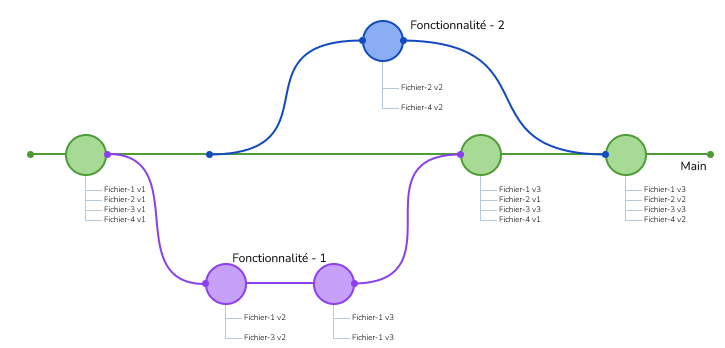
\includegraphics[width=18cm]{Figures/Git.png}
    \caption{Flux d'ajout des fonctionnalités en Git}
\end{figure}

%[width=7cm] you control the size of the image. other options include: 
%[height=7cm] or [scale=0.5] (means half the size of the original image)

\subsection{GitHub}

\begin{itemize}
  \item \textbf{Hébergement du Code: }J'ai hébergé le code source du projet sur GitHub, ce qui m'a permis de le partager facilement avec mes collaborateurs et mon encadrant.
  \item \textbf{Suivi des Problèmes (Issues): }J'ai utilisé la fonctionnalité des Issues sur GitHub pour suivre les tâches, les bogues et les demandes de fonctionnalités tout au long du développement du projet. Les Issues ont permis une communication efficace entre les membres de l'équipe et ont contribué à une gestion transparente des problèmes.
  \item \textbf{Pull Requests (Demandes de Tirage): }Pour intégrer les modifications dans le code principal du projet, j'ai créé des Pull Requests sur GitHub. Les Pull Requests ont facilité la révision du code par les pairs, les tests d'intégration et les validations avant la fusion finale.
\end{itemize}

\begin{figure}[H] 
    \centering
    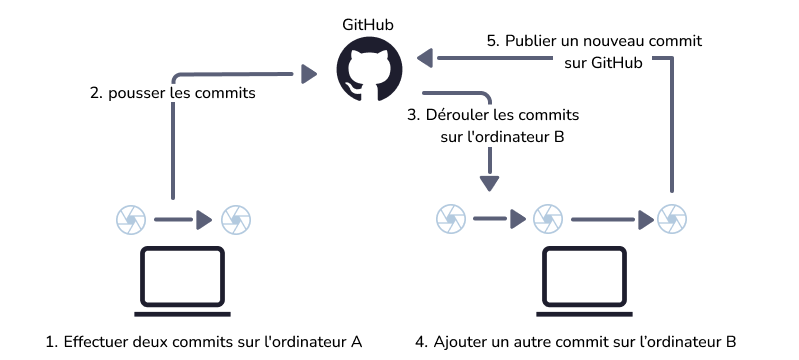
\includegraphics[width=18cm]{Figures/github.png}
    \caption{Collaborer sur github}
\end{figure}

\section{Autres Outils}

\subsection{\LaTeX}

\hspace{16pt}Pour la rédaction du rapport de ce projet, j'ai choisi d'utiliser \LaTeX, un système de composition de documents largement utilisé dans le domaine académique et technique pour sa capacité à produire des documents de haute qualité typographique. \LaTeX\xspace offre de nombreux avantages pour la rédaction de rapports techniques, notamment:

\begin{itemize}
  \item \textbf{Typographie de haute qualité: }\LaTeX\xspace produit des documents avec une typographie professionnelle et esthétique, offrant un rendu précis des symboles mathématiques, des formules, des tableaux et des graphiques.
  \item \textbf{Gestion avancée des références: }\LaTeX\xspace simplifie la gestion des références croisées, des citations bibliographiques et des tableaux des matières, ce qui facilite l'organisation et la navigation dans le rapport.
  \item \textbf{Séparation du contenu et de la mise en page: }\LaTeX\xspace permet de séparer le contenu du document de sa mise en page, ce qui facilite la modification et la réorganisation du contenu sans affecter la présentation visuelle.
\end{itemize}


\subsection{Postman}

\hspace{16pt}Postman a été un outil essentiel dans le processus de développement de l'API pour notre projet. En tant que plateforme de collaboration pour le développement d'API, Postman nous a permis de tester facilement les points de terminaison de notre API RESTful. Avec Postman, nous avons pu envoyer des requêtes HTTP, inspecter les réponses, et valider le comportement de notre API à différentes étapes du développement. L'interface conviviale de Postman nous a également permis de partager nos collections d'API avec d'autres membres de l'équipe et de collaborer efficacement sur les tests et les validations. En résumé, Postman a grandement facilité le processus de développement et de test de notre API, contribuant ainsi à la qualité et à la fiabilité de notre solution logicielle.


\subsection{Eraser}

\hspace{16pt}Eraser a été un élément essentiel de notre processus de conception pour visualiser l'architecture et le flux de notre application. Voici comment nous avons utilisé cet outil:

\begin{itemize}
  \item \textbf{Création de Diagrammes: }Eraser nous a permis de créer des diagrammes de classe, des diagrammes de séquence et d'autres types de schémas pour représenter les différents aspects de notre application.
  \item \textbf{Personnalisation: }Nous avons bénéficié d'une large gamme d'outils et de fonctionnalités offerts par Eraser, nous permettant ainsi de personnaliser nos diagrammes selon nos besoins spécifiques et de les rendre aussi clairs et informatifs que possible.
  \item \textbf{Collaboration: }L'interface intuitive d'Eraser et sa capacité à exporter des diagrammes dans divers formats ont facilité la collaboration au sein de l'équipe. Nous avons pu partager nos diagrammes avec les membres de l'équipe et les parties prenantes pour recueillir des commentaires et assurer une compréhension commune du système.
\end{itemize}


\subsection{Figma}

\hspace{16pt}Figma a été un outil polyvalent dans notre processus de conception, nous permettant de créer à la fois des diagrammes détaillés et des présentations visuellement attrayantes. Voici comment nous l'avons utilisé:

\begin{itemize}
  \item \textbf{Création de Diagrammes: }Comme Eraser, Figma nous a permis de créer des diagrammes de classe, des diagrammes de séquence et d'autres types de schémas pour représenter l'architecture et le flux de notre application. Nous avons bénéficié d'une interface conviviale et d'outils intuitifs pour réaliser ces diagrammes avec précision.
  \item \textbf{Présentations Visuelles: }En plus de la création de diagrammes, Figma a également été utilisé pour créer des présentations visuellement attrayantes. Nous avons pu intégrer des diagrammes, des maquettes d'interface utilisateur et d'autres éléments visuels dans nos présentations pour communiquer efficacement nos idées et nos concepts.
\end{itemize}

\newpage

\section*{Conclusion}


\hspace{16pt}Ce chapitre a couvert les différents composants de l'environnement de développement, incluant Arch Linux comme système d'exploitation, Neovim pour l'édition de texte, Alacritty comme terminal, et Git pour le contrôle de version. Chaque choix a été justifié par ses avantages spécifiques pour le projet.


\chapter{Conception et développement de l’application}
\label{chap:Chapter 3 title}
\section*{Introduction}

\hspace{16pt}Ce chapitre se concentre sur la conception et le développement de l'application. Nous commencerons par une description détaillée du flux de l'application, en expliquant comment elle guide les utilisateurs à travers ses différentes fonctionnalités. Ensuite, nous aborderons les choix technologiques majeurs, notamment l'utilisation de React pour l'interface utilisateur et Symfony pour le backend. Enfin, nous présenterons les diagrammes de conception utilisés pour visualiser et planifier l'architecture de l'application.

\newpage


\section{Description du flux de Chatbot}

\hspace{16pt}Le flux de l'application du chatbot pour la maison médicale se déroule en plusieurs étapes clés, organisées pour optimiser l'expérience utilisateur:

\begin{figure}[H] 
    \centering
    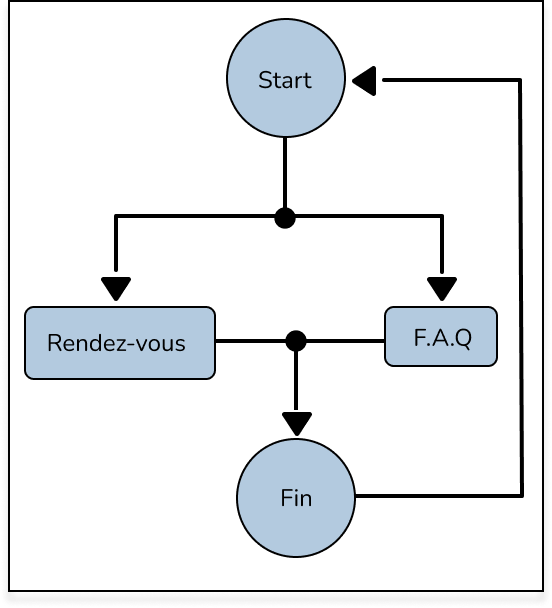
\includegraphics[scale=0.8]{Figures/cbf_overall.png}
    \caption{Flux général du Chatbot}
\end{figure}

% [width=8cm]
\subsection{FAQ}

\hspace{16pt}Le chatbot propose à l'utilisateur des sujets prédéfinis sur lesquels il pourrait vouloir en savoir plus, et lors de la sélection d'un, le chatbot répond avec une réponse prédéfinie.

\begin{figure}[H] 
    \centering
    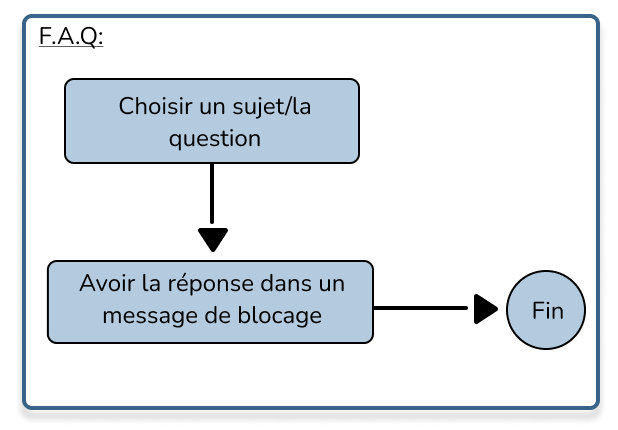
\includegraphics[scale=0.8]{Figures/cbf_faq.png}
    \caption{Flux du processus: F.A.Q}
\end{figure}

\subsection{Prise de rendez-vous}

\hspace{16pt}Le chatbot guide l'utilisateur avec un flux prédéfini dans ce cas, depuis la demande d'informations de base sur l'utilisateur jusqu'aux opérations facultatives telles que répondre à des questions spécialisées ou joindre des documents, avec une validation intégrée pour chaque petite information que nous lui demandons de fournir (si la validation est possible dans le premier lieu).


\begin{figure}[H] 
    \centering
    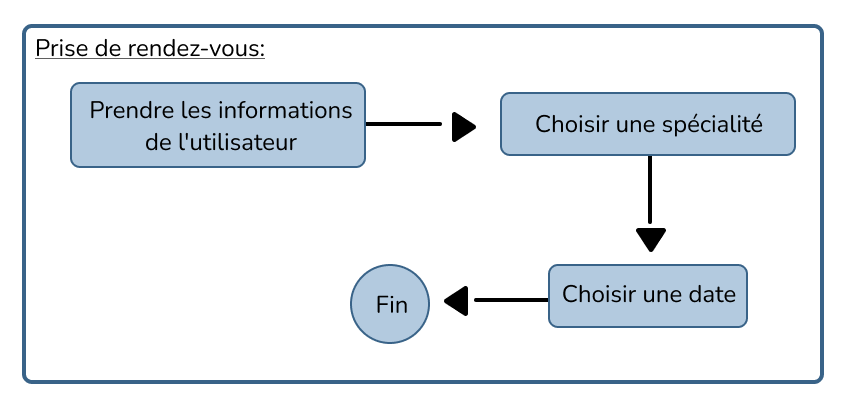
\includegraphics[scale=0.8]{Figures/cbf_rdv.png}
    \caption{Flux du processus: Prise de rendez-vous}
\end{figure}


\begin{figure}[H] 
    \centering
    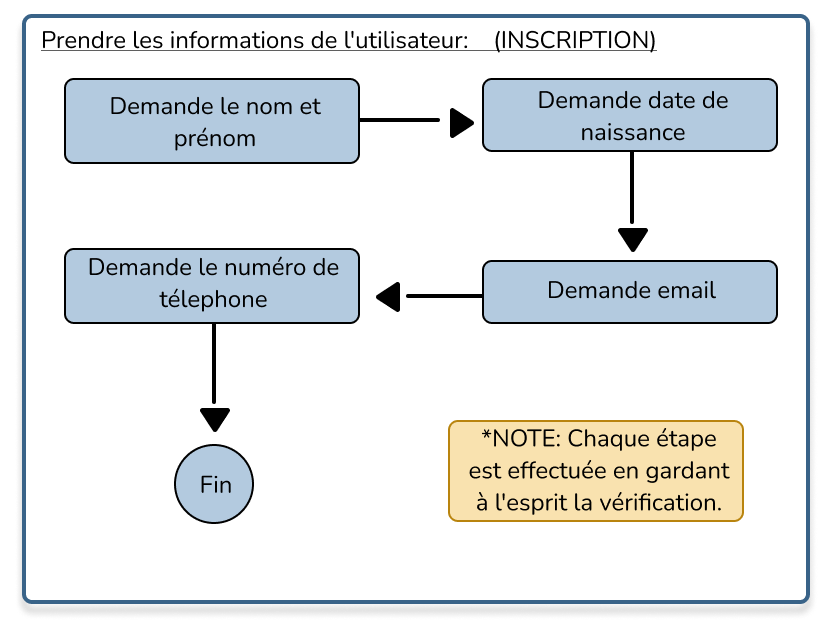
\includegraphics[scale=0.8]{Figures/cbf_user.png}
    \caption{Flux du processus: Prise de rendez-vous (Prendre les informations de l'utilisateur)}
\end{figure}


\begin{figure}[H] 
    \centering
    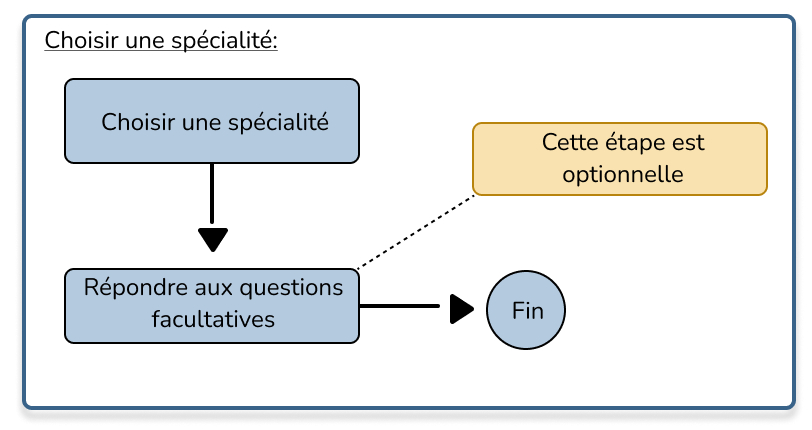
\includegraphics[scale=0.9]{Figures/cbf_specialite.png}
    \caption{Flux du processus: Prise de rendez-vous (Choisir une spécialité)}
\end{figure}


\section{Explication des choix technologiques}

\hspace{16pt}Pour les technologies, nous n'avions pas beaucoup de choix, on nous proposait de travailler soit avec Django de Python, soit avec React (Front-end) et Symfony* (Back-end).

\subsection{React}


\subsubsection{Interface Utilisateur Réactive et Performante}

\begin{itemize}
  \item \textbf{DOM Virtuel: }React utilise un DOM virtuel pour des mises à jour rapides et efficaces de l'interface utilisateur, garantissant une expérience utilisateur fluide et sans latence.
  \item \textbf{Rendu Dynamique: }Les capacités de rendu dynamique de React permettent de gérer efficacement les interactions en temps réel, cruciales pour un chatbot.
\end{itemize}

\subsubsection{Composants Réutilisables et Modulaire}
 
\begin{itemize}
  \item \textbf{Composants: }La structure basée sur les composants de React facilite la création de widgets et de modules réutilisables pour différentes parties du chatbot, comme les fenêtres de conversation, les formulaires de saisie, et les notifications.
  \item \textbf{Modularité: }Permet de construire l'application de manière modulaire, rendant le code plus maintenable et évolutif.
\end{itemize}

\subsubsection{Intégration Facile avec les APIs}

\begin{itemize}
  \item \textbf{Hooks: }Les hooks de React, comme useEffect et useState, simplifient les appels API et la gestion des états, permettant une intégration fluide avec les services backend du chatbot.
  \item \textbf{Interopérabilité: }React facilite l'intégration avec des APIs RESTful ou GraphQL, nécessaires pour les fonctionnalités de traitement du langage naturel (NLP) et la gestion des dialogues.
\end{itemize}

\subsubsection{Écosystème et Communauté}

\begin{itemize}
  \item \textbf{Support et Documentation: }La vaste communauté de React et sa documentation exhaustive offrent un soutien continu et des ressources abondantes pour résoudre les problèmes et optimiser le développement.
  \item \textbf{Outils et Bibliothèques: }Un large éventail de bibliothèques et d'outils complémentaires, tels que les bibliothèques de calendriers et même la bibliothèque de chatbots avec laquelle nous avons travaillé.
\end{itemize}


\subsection{Symfony}


\subsubsection{Framework PHP Puissant}

\begin{itemize}
  \item Symfony est un framework PHP mature et puissant, offrant une structure solide et bien organisée pour le développement d'applications web complexes telles que le chatbot médical. Sa stabilité et sa maturité en font un choix fiable pour la création d'un back-end robuste.
\end{itemize}

\subsubsection{Gestion de l'API avec API Platform}

\begin{itemize}
  \item Symfony offre une intégration transparente avec API Platform, une solution robuste pour la création et la gestion d'API RESTful. En configurant l'API avec Symfony et API Platform, nous bénéficions d'une documentation automatique, d'une gestion avancée des opérations CRUD, et d'une sérialisation/désérialisation automatique des données.
\end{itemize}

\subsubsection{Sécurité Renforcée}

\begin{itemize}
  \item Symfony intègre des fonctionnalités avancées de sécurité, telles que la protection contre les attaques CSRF, XSS et SQL injection. Cela garantit un niveau élevé de sécurité pour les données sensibles des utilisateurs du chatbot médical, ce qui est essentiel dans le domaine médical.
\end{itemize}


\section{Diagrammes de conception utilisés}

\hspace{16pt}Dans le cadre du développement du chatbot pour la maison médicale, nous avons créé un Modèle Conceptuel de Données (MCD) pour concevoir la structure de la base de données. Le MCD ci-dessous illustre les principales entités et leurs relations dans notre système.\\


\begin{figure}[H] 
    \centering
    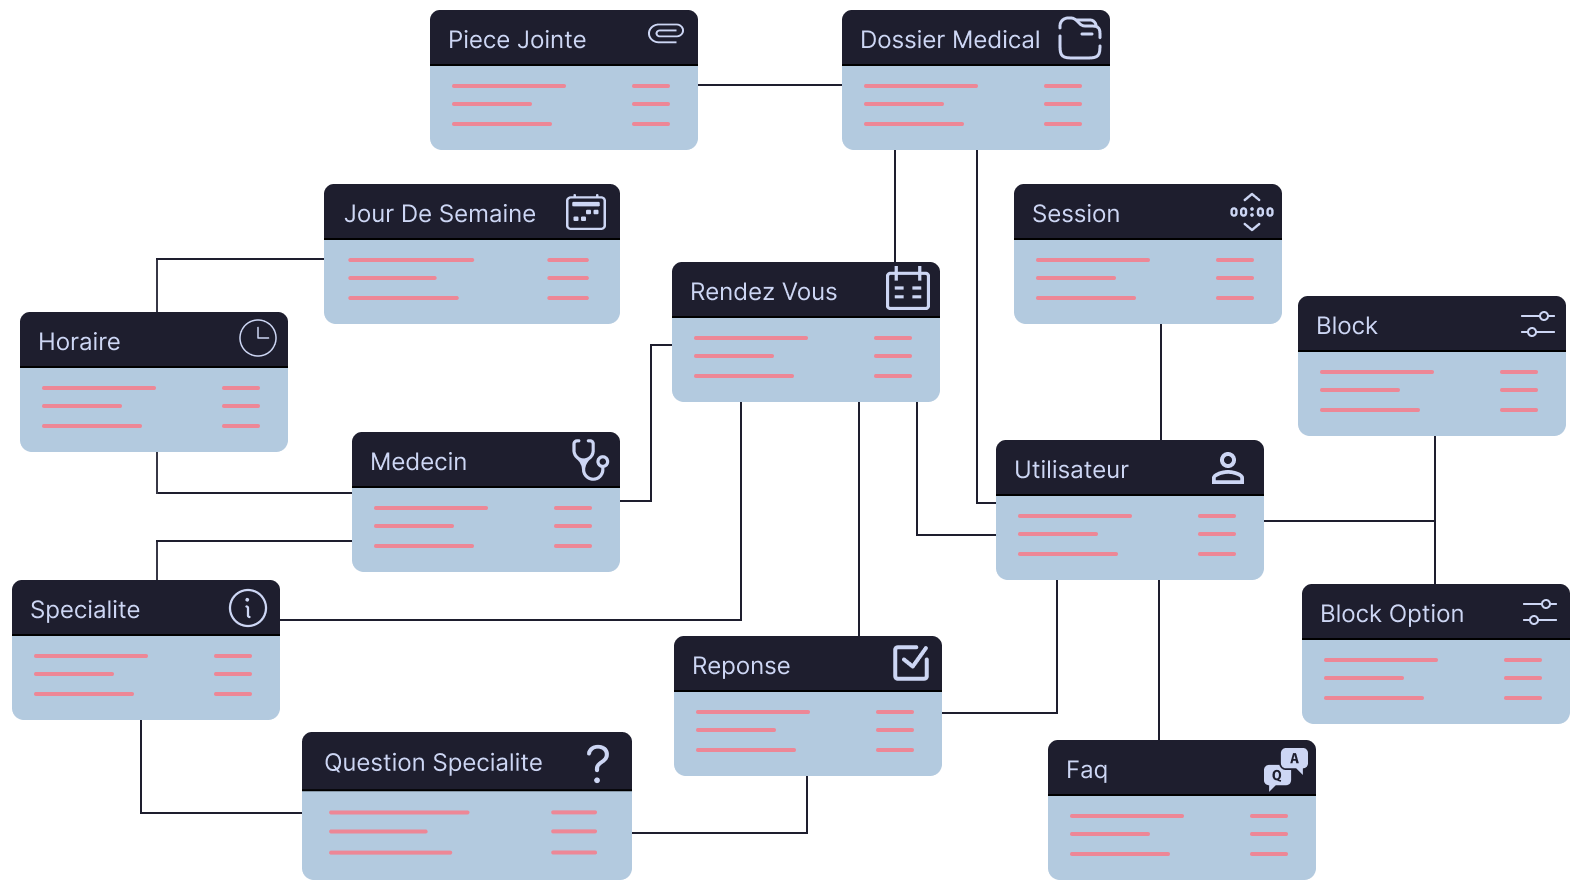
\includegraphics[scale=0.67]{Figures/MCD.png}
    \caption{Diagramme de conception}
    \label{entite} %Optional (If you want to reference the figure in later chapters)
\end{figure}

Ce MCD représente les principales entités de notre base de données pour le chatbot médical. Voici une brève explication de chaque entité :


\begin{itemize}
  \item \textbf{Utilisateur: }Stocke les informations sur les utilisateurs du chatbot, telles que leur identifiant, leur nom et leurs informations de contact. Les utilisateurs peuvent avoir des rôles spécifiques, comme patient ou admin.
  \item \textbf{Medecin: }Stocke les informations sur les médecins, telles que leur identifiant, leur nom et leurs informations de contact.
  \item \textbf{Specialite: }Décrit les différentes spécialités médicales disponibles, telles que la cardiologie, la dermatologie, etc.
  \item \textbf{Question Specialite: }Contient des questions uniques pour chaque spécialité.
  \item \textbf{Reponse: }Enregistre les réponses fournies par les patients aux questions relatives à une spécialité médicale. Inclut des références à l'utilisateur, à la question de spécialité et à la réponse fournie.
  \item \textbf{Jour De Semaine: }Stocke les jours de la semaine pour aider à gérer les horaires et les disponibilités des médecins et des rendez-vous.
  \item \textbf{Horaire: }Définit les plages horaires disponibles pour les rendez-vous et les sessions avec les médecins.
  \item \textbf{Session: }Contient la séance de travail pour le centre médical.
  \item \textbf{Rendez Vous: }Enregistre les rendez-vous programmés, y compris la date, l'heure, le patient et le médecin assigné.
  \item \textbf{Faq: }Stocke les questions fréquentes et leurs réponses associées, utilisées par le chatbot pour fournir des informations instantanées.
  \item \textbf{Block: }Décrit les blocs de contenu ou de dialogue utilisés dans le chatbot pour structurer les conversations.
  \item \textbf{Block Option: }Contient les options disponibles pour chaque bloc de contenu, permettant au chatbot de guider les utilisateurs à travers différentes branches de la conversation.
  \item \textbf{Piece jointe: }Gère le téléchargement de fichiers. Cette entité stocke les informations sur les fichiers joints aux conversations.
  \item \textbf{Dossier Medical: }Gère les dossiers médicaux des utilisateurs. Cette entité permet le téléchargement de plusieurs fichiers pour chaque utilisateur.
\end{itemize}



\newpage

\section*{Conclusion}

\hspace{16pt}La conception et le développement de l'application décrits dans ce chapitre montrent comment les choix technologiques et les approches méthodologiques ont permis de créer une solution efficace et robuste. En utilisant des frameworks modernes et des pratiques de conception bien établies, nous avons pu développer une application qui répond aux besoins des utilisateurs de manière optimale.

\pagebreak


\chapter{Les missions effectuées}
\label{chap:Chapter 4 title}
\section*{Introduction}

\hspace{16pt}Ce chapitre est consacré à la description des missions effectuées durant le stage. Chaque mission représente une étape clé dans le développement du chatbot, depuis la configuration initiale jusqu'à la mise en ligne. Nous aborderons la configuration des environnements de développement, la création et la gestion des bases de données, et le développement des interfaces utilisateur. En détaillant ces missions, nous mettrons en lumière les compétences techniques mobilisées et les défis rencontrés. Ce chapitre vise à illustrer le processus de développement et les contributions spécifiques apportées à chaque étape du projet.

\pagebreak

\section{Le Chatbot}

\subsection{Configuration static}

\hspace{16pt}La configuration statique du chatbot concerne les éléments du chatbot qui sont définis à l'avance et qui ne changent pas dynamiquement en fonction des interactions utilisateur. Voici quelques aspects clés de cette configuration:

\begin{itemize}
  \item \textbf{Réponses prédéfinies: }Le chatbot est programmé avec une série de réponses prédéfinies pour les questions fréquentes.
  \item \textbf{Flow du prise de rendez-vous: }Définir un flux statique qui accompagnera l'utilisateur dans sa prise de rendez-vous.
  \item \textbf{Interface utilisateur: }La présentation et les options initiales du chatbot, telles que les boutons de démarrage et les messages de bienvenue, sont configurées statiquement.
  \item \textbf{Connexion: }Configurer un processus statique permettant aux utilisateurs de se connecter avant d'utiliser certaines fonctionnalités du chatbot.
  \item \textbf{Inscription: }Mettre en place un processus d'inscription statique pour les nouveaux utilisateurs, leur permettant de créer un compte avant d'accéder aux fonctionnalités du chatbot.
\end{itemize}

\begin{figure}[H] 
    \centering
    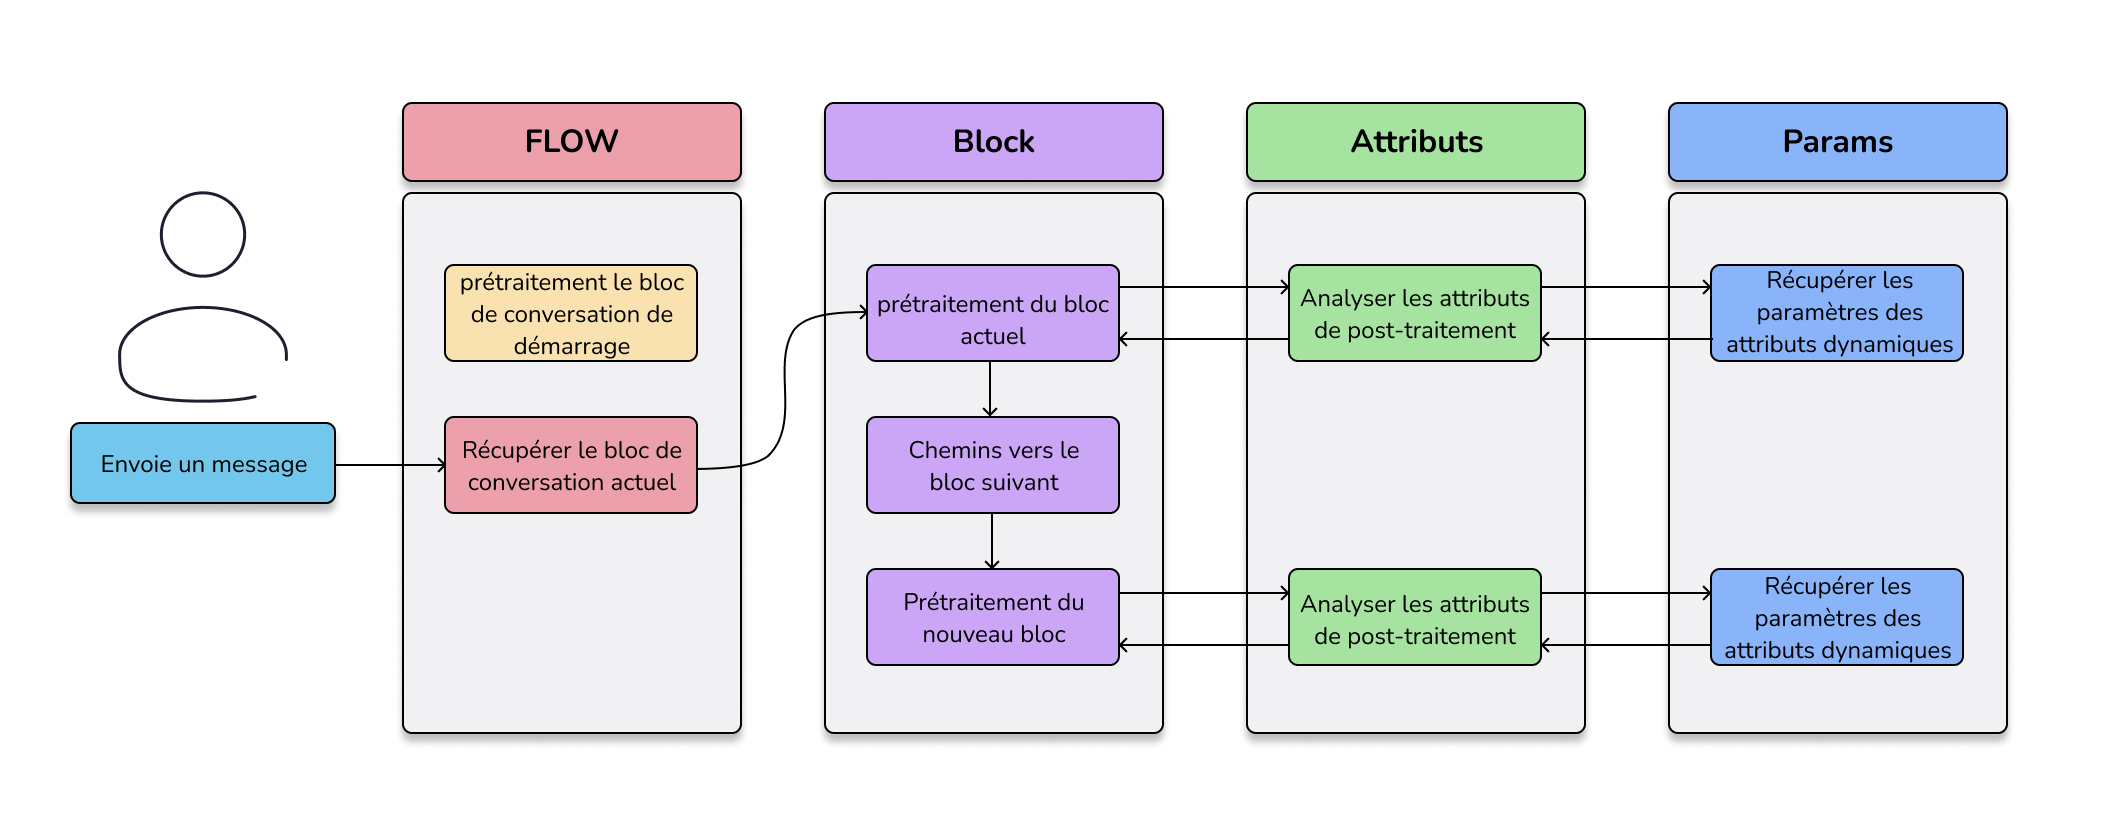
\includegraphics[scale=0.5]{Figures/chatbot.png}
    \caption{Structure générale du configuration Chatbot}
\end{figure}

\subsection{Configuration dynamique}

\hspace{16pt}Concernant les aspects dynamiques de notre chatbot, il nous a été demandé de le rendre « entièrement » personnalisable, ce qui signifie:

\begin{itemize}
  \item \textbf{Construction dynamique: }Chaque message à l'écran doit être configurable via un tableau de bord, y compris les messages d'erreur.
  \item \textbf{Messages dynamiques: }Les messages doivent être modifiés en fonction du contexte.
  \item \textbf{Flux dynamique: }L'utilisateur doit avoir la possibilité de choisir entre où aller ensuite à partir de sa position actuelle (à l'exclusion bien sûr des flux dans lesquels nous demandons des informations critiques pour créer le compte de l'utilisateur)
  \item \textbf{Composant dynamique: }Les composants personnalisés doivent s'adapter aux entrées de l'utili-sateur et afficher les informations en conséquence.
  \item \textbf{Données dynamiques: }chaque information contenue par le chatbot provient de l'API qui connecte notre chatbot à la base de données.
\end{itemize}


\begin{figure}[H] 
    \centering
    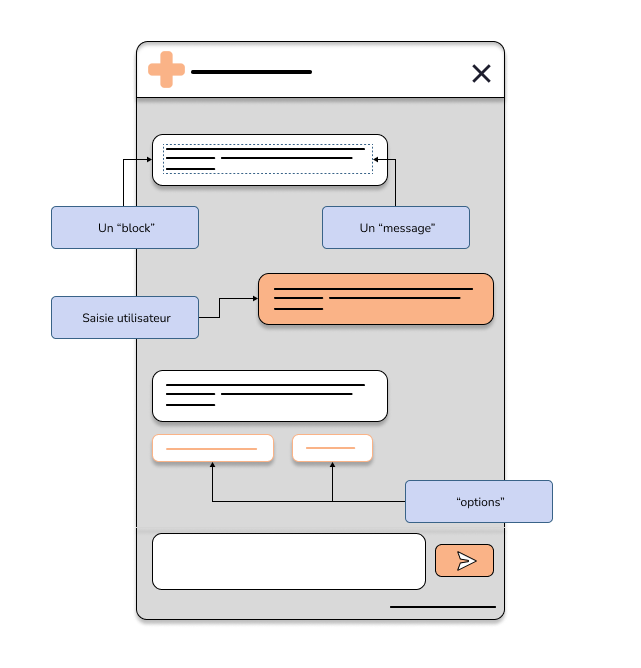
\includegraphics[scale=0.5]{Figures/cbs_general.png}
    \caption{Structure générale du Chatbot}
\end{figure}


\begin{figure}[H] 
    \centering
    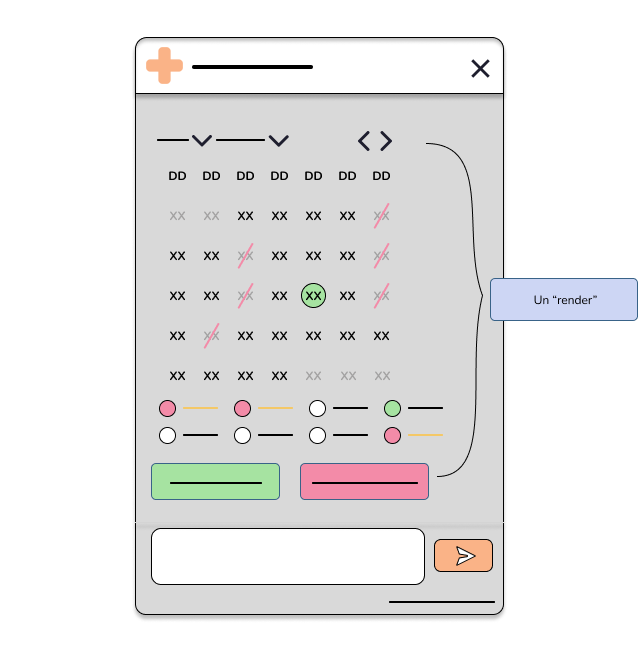
\includegraphics[scale=0.5]{Figures/cbs_render.png}
    \caption{Structure générale du Chatbot (exemple de "render" element)}
\end{figure}

\section{La base de donnéés}


\subsection{Création des entités}

\hspace{16pt}La création des entité (Figure \ref{entite}) dans la base de données est une étape cruciale pour structurer les informations de manière efficace et logique.

En structurant ces entités de manière logique et efficace, nous avons pu créer une base de données robuste et évolutive, capable de gérer les différentes facettes du projet, y compris la gestion des utilisateurs, des médecins, des rendez-vous, et des interactions du chatbot.

\subsection{Configuration d'API}

\hspace{16pt}Une API (Application Programming Interface) est un ensemble de règles permettant à des applications de communiquer entre elles. Elle utilise des protocoles comme HTTP/HTTPS pour échanger des données et donne accès à certaines fonctionnalités ou informations d'un service.

\begin{figure}[H] 
    \centering
    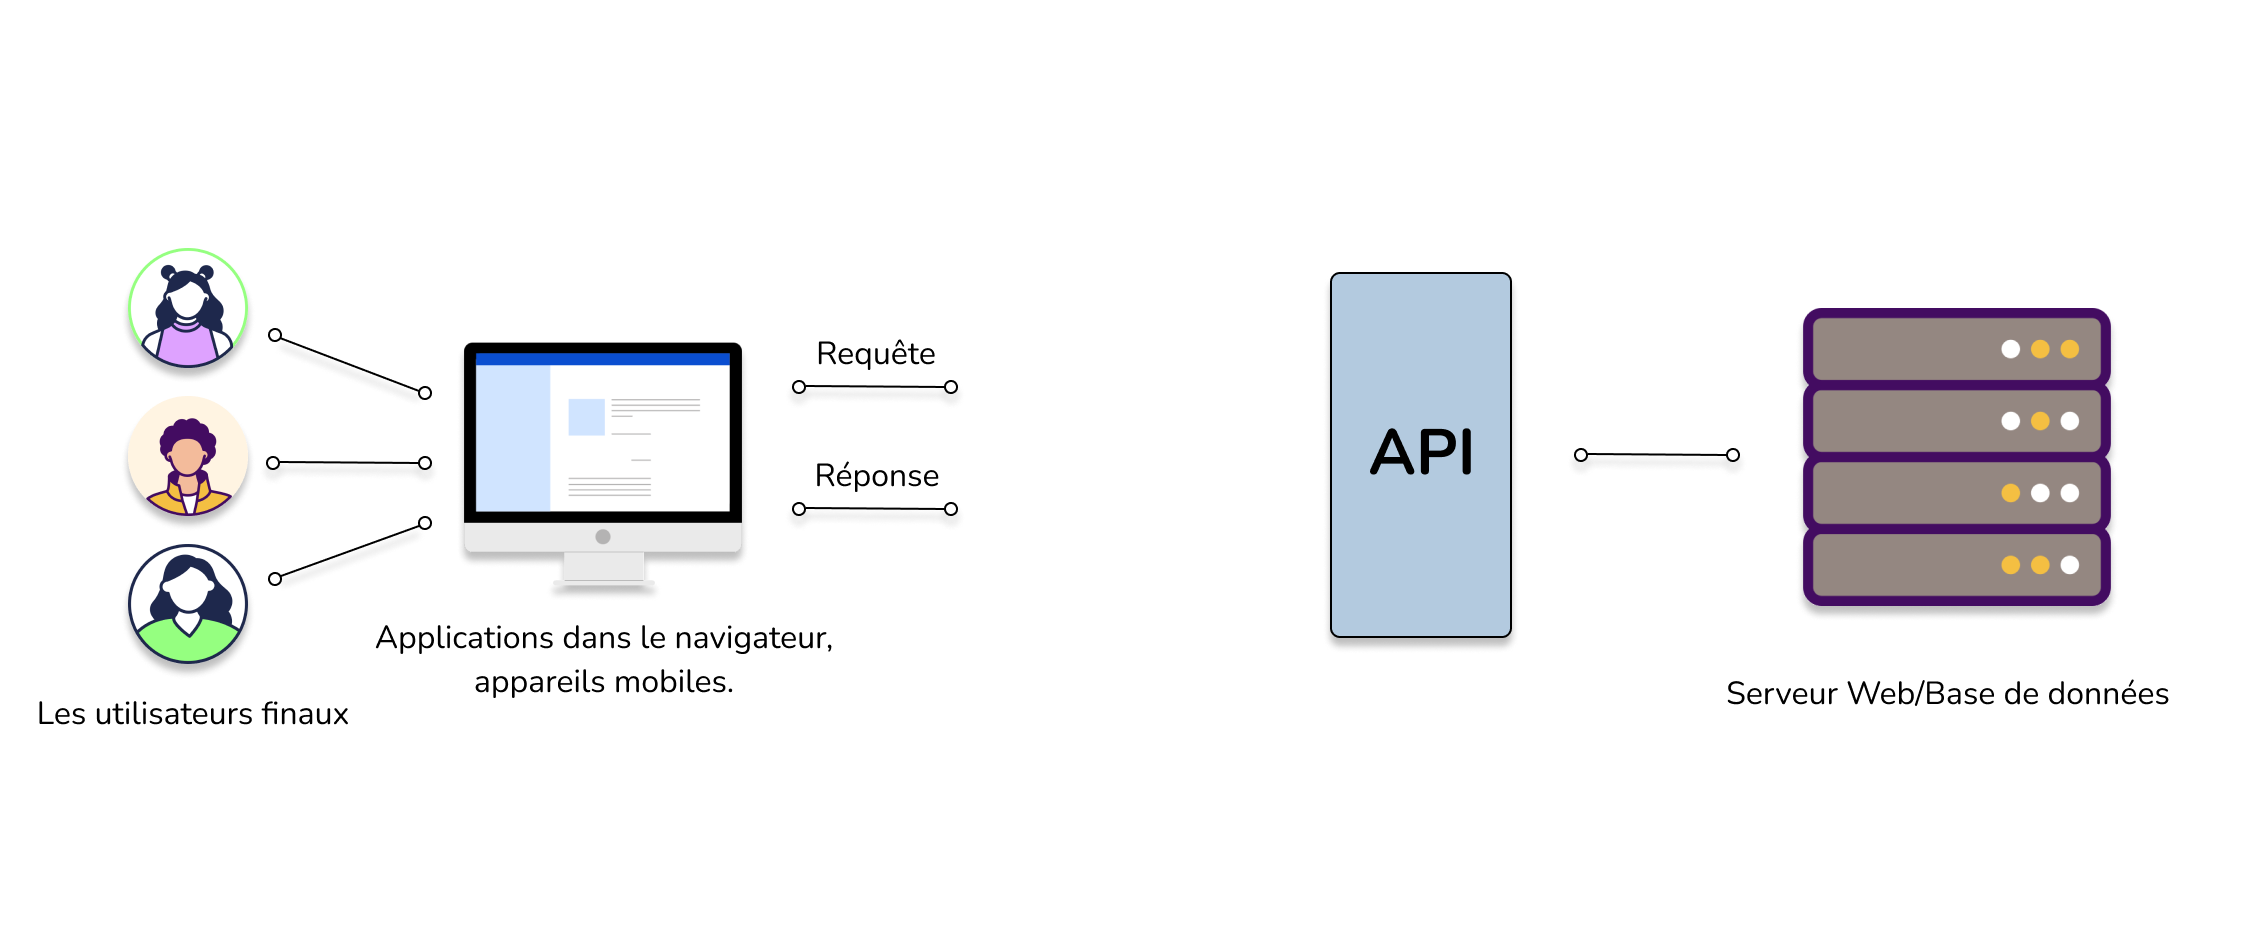
\includegraphics[scale=0.49]{Figures/API.png}
    \caption{Foncionnement d'un API}
\end{figure}

La configuration de l'API est une étape essentielle pour permettre une communication efficace entre le frontend et le backend de notre application.

Pour ce projet, nous avons utilisé Symfony avec API Platform pour créer une API RESTful. API Platform offre une grande flexibilité et permet de configurer facilement les opérations CRUD (Create, Read, Update, Delete), la validation des champs, la gestion des relations, les filtres et les groupes de sérialisation. Voici un aperçu de ces fonctionnalités:

\begin{itemize}
  \item \textbf{Opérations CRUD Configurables: }API Platform facilite la configuration des opérations CRUD pour chaque entité. Par défaut, les opérations GET, POST, PUT, DELETE sont disponibles, mais elles peuvent être personnalisées ou restreintes selon les besoins.
  \item \textbf{Validation des Champs: }API Platform intègre le composant de validation de Symfony, ce qui permet de définir des règles de validation directement dans les entités.
  \item \textbf{La gestion des relations entre les entités est simplifiée avec API Platform. Les relations peuvent être configurées pour être exposées via l'API.}
  \item \textbf{API Platform permet d'ajouter facilement des filtres pour les opérations GET. Ces filtres permettent de rechercher et de trier les données de manière flexible.}
  \item \textbf{Groupes de Sérialisation: }Les groupes de sérialisation permettent de contrôler les données qui sont exposées via l'API. Cela est utile pour restreindre les champs visibles selon le contexte (lecture, écriture, etc.).
\end{itemize}

\begin{figure}[H] 
    \centering
    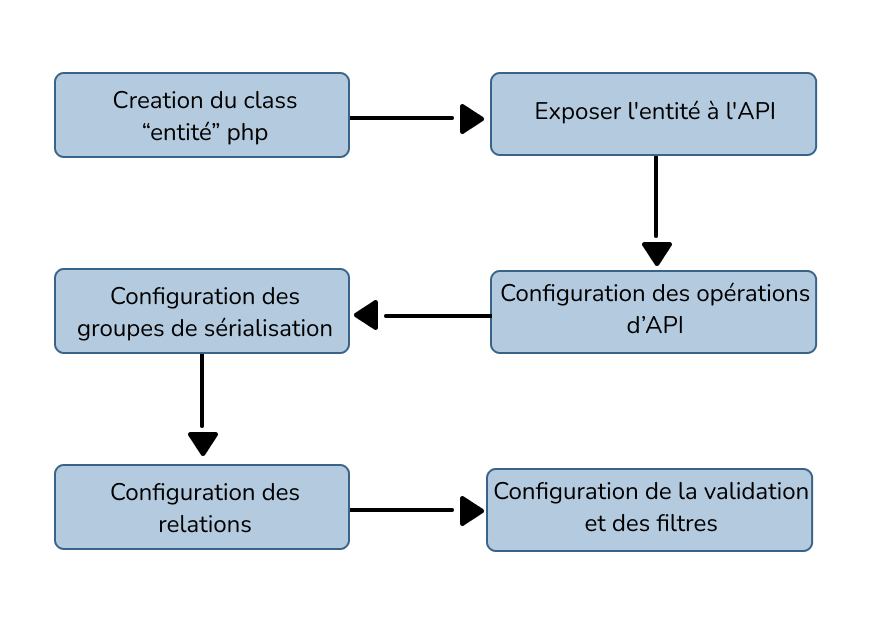
\includegraphics[scale=0.9]{Figures/api_entity.png}
    \caption{Flux général de création d'une entité API}
\end{figure}

\section{Tableau de bord}

\subsection{La gestion des rendez-vous}

\hspace {16pt}La gestion des rendez-vous est une fonctionnalité essentielle du dashboard, permettant aux admini-strateurs et aux médecins de suivre et de gérer efficacement les consultations des patients. Voici les principales caractéristiques de cette fonctionnalité:

\begin{itemize}
  \item \textbf{Vue Calendrier: }Une interface calendrier permet de visualiser les rendez-vous par jour, semaine ou mois. Les rendez-vous sont colorés en fonction de leur statut (confirmé, en attente, annulé).
  \item \textbf{Confirmation et Modification: }Les administrateurs peuvent confirmer, modifier ou annuler des rendez-vous directement depuis le dashboard.
\end{itemize}

\subsection{La gestion d'équipe medicale}

\hspace{16pt} La gestion de l’équipe médicale est une autre fonctionnalité clé du dashboard, assurant une organi-sation optimale des ressources humaines et des services offerts. Voici comment cette fonctionnalité est mise en œuvre:

\begin{itemize}
  \item \textbf{Liste des Médecins: }Une liste détaillée des médecins avec leurs spécialités, disponibilités et coordonnées. Les administrateurs peuvent facilement ajouter, modifier ou désactiver des médecins.
  \item \textbf{Planification des Horaires: }Un module de planification permet de définir les horaires de travail des médecins.
  \item \textbf{Gestion des Spécialités: }Les administrateurs peuvent gérer les spécialités médicales, en ajoutant ou supprimant des spécialités et en assignant des médecins aux différentes spécialités.
  \item \textbf{Rapports et Statistiques: }Des rapports détaillés sur les activités des médecins, incluant le nombre de consultations, le taux de satisfaction des patients, et les performances par spécialité.
\end{itemize}

\subsection{La gestion du Chatbot}

\hspace{16pt} La gestion du chatbot depuis le dashboard permet de maintenir et d’améliorer en continu l’interaction avec les patients. Voici les fonctionnalités principales de cette section:

\begin{itemize}
  \item \textbf{Configuration des F.A.Q: }Les administrateurs peuvent ajouter ou modifier les réponses pré-définies du chatbot pour les questions fréquentes. Cela inclut la mise à jour des informations sur les horaires, les services et les procédures.
  \item \textbf{Personnalisation: }Des options de personnalisation permettent de modifier le comportement du chatbot, incluant les messages de bienvenue.
\end{itemize}

\newpage

\section*{Conclusion}

\hspace{16pt}En conclusion, les missions effectuées ont permis de mettre en pratique une large gamme de compé-tences techniques et organisationnelles. Chaque étape du projet a été l'occasion d'apprendre et de s'adapter, démontrant la complexité et la richesse du processus de développement. Les compétences acquises et les défis surmontés ont non seulement contribué à la réussite du projet, mais ont également enrichi notre expérience professionnelle de manière significative.

\pagebreak


\chapter{Les apports du stage}
\label{chap:Chapter 5 title} 
\section*{Introduction}

\hspace{16pt}Le stage chez FCPO a été une expérience riche en apprentissages et en développement professionnel. Ce chapitre examine les différents apports du stage, tant sur le plan théorique qu'intellectuel et pratique. Nous aborderons les compétences techniques acquises, les connaissances théoriques consolidées, et les leçons tirées de l'intégration dans une équipe professionnelle. L'expérience de la gestion de projet et l'application concrète des technologies avancées ont joué un rôle crucial dans notre formation. Ce chapitre vise à offrir une réflexion sur la valeur ajoutée de cette expérience de stage et son impact sur notre développement professionnel.

\pagebreak

\section{Les apports théoriques et intellectuels}

\hspace{16pt} Durant ce stage, j’ai pu approfondir plusieurs concepts théoriques que j'avais appris lors de ma formation académique. Les principaux apports théoriques et intellectuels incluent:

\begin{itemize}
  \item \textbf{Architecture des applications web: }J’ai consolidé mes connaissances sur les architectures MVC (Model-View-Controller) en travaillant avec Symfony et API Platform. J’ai appris à structurer efficacement une application web pour assurer une bonne séparation des préoccupations et une maintenance facile.
  \item \textbf{Systèmes de gestion de bases de données: }J’ai approfondi mes compétences en conception et gestion de bases de données relationnelles, en particulier avec MySQL. J’ai appris à modéliser des entités complexes et à gérer les relations entre elles de manière optimale.
\end{itemize}

\section{Les compétences pratiques développées}

\hspace{16pt}Le stage m’a offert l’opportunité de développer et de perfectionner des compétences pratiques essentielles pour un développeur. Les compétences pratiques acquises comprennent:

\begin{itemize}
  \item \textbf{Développement Frontend avec React: } J’ai amélioré mes compétences en développement frontend en utilisant React pour créer des interfaces utilisateur interactives et réactives.
  \item \textbf{Développement Backend avec Symfony et API Platform: }J’ai acquis une expérience pratique significative en utilisant Symfony pour le développement backend et API Platform pour la création d’APIs RESTful. J’ai appris à configurer des opérations CRUD, à valider des champs et à gérer des relations entre entités.
  \item \textbf{Gestion de version avec Git et GitHub: }J’ai perfectionné mes compétences en gestion de version avec Git, en utilisant GitHub pour collaborer avec les membres de l’équipe, gérer des branches, résoudre des conflits et suivre l’historique des modifications.
  \item \textbf{Utilisation d’outils de développement: }J’ai optimisé mon environnement de développement en utilisant Arch Linux, Neovim avec une configuration personnalisée, et des outils comme Alacritty, ZSH, tmux, et fzf. Cela m’a permis de travailler de manière plus efficace et productive.
\end{itemize}

\section{Les apports en termes de monde de l'entreprise}

\hspace{16pt}Ce stage m’a également offert une précieuse perspective sur le fonctionnement et la culture d’entreprise. Voici quelques apports significatifs:

\begin{itemize}
  \item \textbf{Travail en équipe: }J’ai appris à collaborer efficacement avec une équipe de développeurs, à communiquer clairement, à partager des tâches et à résoudre des problèmes ensemble. J’ai compris l’importance de la coordination et de la coopération dans la réussite d’un projet.
  \item \textbf{Gestion de projet: }J’ai été exposé aux méthodologies de gestion de projet agile, telles que les sprints et les réunions quotidiennes. J’ai appris à gérer mon temps, à prioriser les tâches et à respecter les délais tout en assurant la qualité du travail.
  \item \textbf{Adaptation aux exigences des clients: }J’ai acquis une meilleure compréhension de l’importance de répondre aux besoins des clients et de s’adapter rapidement aux changements de spécifications. J’ai appris à être flexible et réactif pour fournir des solutions qui satisfont les attentes des utilisateurs finaux.
  \item \textbf{Culture d’entreprise et éthique professionnelle: }J’ai intégré les valeurs et les pratiques professionnelles de FCPO, telles que le respect des délais, la qualité du travail, la confidentialité des données et l’engagement envers les objectifs de l’entreprise. Cela m’a permis de développer un sens aigu de la responsabilité et de l’éthique professionnelle.
\end{itemize}


\newpage
\section*{Conclusion}

\hspace{16pt}Les apports du stage chez FCPO sont nombreux et variés. Sur le plan théorique, ce stage a permis de consolider les connaissances acquises au cours de nos études, tout en les appliquant à des situations réelles et complexes. Sur le plan pratique, nous avons développé des compétences techniques avancées, appris à naviguer dans un environnement professionnel exigeant, et à collaborer efficacement au sein d'une équipe. Cette expérience a été formatrice à bien des égards, renforçant notre confiance en nos capacités et nous préparant à affronter les défis futurs avec assurance et compétence.


\chapter{Les difficultés du stage et les solutions apportées}
\label{chap:Chapter 6 title} 
\section*{Introduction}

Lorem ipsum dolor sit amet, consectetur adipiscing elit. Praesent nec dapibus justo. Donec sagittis vulputate ante sed porttitor. Suspendisse sit amet nisl massa. Curabitur nec nisl condimentum, egestas ex vitae, dapibus enim. Etiam iaculis, erat faucibus pellentesque sagittis, nisi justo sollicitudin nibh, et condimentum augue massa non turpis. Proin commodo enim fermentum suscipit condimentum. Maecenas molestie, dui nec vestibulum rhoncus, arcu nisl faucibus neque, a ornare nisi massa ac eros. Aenean id velit sit amet lacus mattis varius. Donec fringilla massa sed nisi eleifend, a aliquet mi tempus. Nunc posuere euismod est, nec tristique augue lobortis non. Sed sodales sem ut metus tempus ullamcorper.

\pagebreak

\section{Les difficultés rencontrées}


\section{Les solutions apportées à ces difficultés}




\newpage
\section*{Conclusion}

Lorem ipsum dolor sit amet, consectetur adipiscing elit. Praesent nec dapibus justo. Donec sagittis vulputate ante sed porttitor. Suspendisse sit amet nisl massa. Curabitur nec nisl condimentum, egestas ex vitae, dapibus enim. Etiam iaculis, erat faucibus pellentesque sagittis, nisi justo sollicitudin nibh, et condimentum augue massa non turpis. Proin commodo enim fermentum suscipit condimentum. Maecenas molestie, dui nec vestibulum rhoncus, arcu nisl faucibus neque, a ornare nisi massa ac eros. Aenean id velit sit amet lacus mattis varius. Donec fringilla massa sed nisi eleifend, a aliquet mi tempus. Nunc posuere euismod est, nec tristique augue lobortis non. Sed sodales sem ut metus tempus ullamcorper.


\chapter*{Conclusion générale et perspectives}


% This conclusion is unnumbered, if you want it numbered, you can remove the * from above and remove the line below, so it becomes a chapter, then add sections.

\addcontentsline{toc}{chapter}{Conclusion générale et perspectives} %adds to the table of contents 

\label{chap:General Conclusion} 

\hspace{16pt}Le stage chez FCPO a été une expérience extrêmement enrichissante et formatrice. Il m'a permis de mettre en pratique les connaissances acquises durant mes études tout en développant de nouvelles compétences dans un cadre professionnel exigeant. Les défis rencontrés ont été nombreux et variés, couvrant des aspects techniques, organisationnels et interpersonnels. Cependant, chaque difficulté a été une occasion d'apprentissage et d'amélioration continue.

Le projet de développement du chatbot pour une maison médicale a été un véritable test de mes capacités à utiliser des technologies avancées telles que Symfony, API Platform et React. La découverte et la maîtrise de ces outils, initialement intimidants, se sont avérées être des atouts précieux pour le projet. Le processus de configuration dynamique du chatbot, en particulier, m'a permis de comprendre l'importance de la conception soignée et de l'optimisation des réponses pour créer une solution interactive et réactive.

L'intégration des différentes entités dans la base de données, ainsi que la configuration des API, a mis en lumière l'importance de la structuration des données et de la gestion des relations entre celles-ci. Grâce à cela, j'ai pu développer une compréhension approfondie de la conception et de l'implémentation de systèmes de gestion de contenu robustes et évolutifs.

En termes de développement personnel, ce stage m'a permis de renforcer mes compétences en résolution de problèmes et en gestion de projet. J'ai appris à travailler efficacement en équipe, à communiquer de manière claire et concise, et à gérer mon temps de manière optimale.

Enfin, ce stage m'a également offert une vision précieuse du monde de l'entreprise. J'ai pu observer de près comment une agence digitale comme FCPO fonctionne, de la gestion des projets à la relation avec les clients. J'ai compris l'importance de la rigueur et de la qualité dans le travail, ainsi que la nécessité de toujours chercher à innover et à s'améliorer.

En conclusion, ce stage a été une étape cruciale dans mon parcours professionnel. Les défis surmontés et les solutions apportées m'ont préparé à aborder avec confiance les futurs projets. Je suis reconnaissant pour cette opportunité et impatient de développer ces compétences dans les projets à venir.



%\section{Optional Section}


% Redefine the appendix name
\renewcommand{\appendixname}{Annexe}

\appendix


\chapter{Glossaire}
\label{chap:Glossary} 


\hspace{16pt}\textbf{Chatbot: }Un programme d'intelligence artificielle qui simule une conversation humaine.\\

\textbf{Arch Linux: }Une distribution Linux simple et légère.\\

\textbf{KISS: }Keep It Simple, Stupid (Garde-le simple, stupide), un principe de conception affirmant que les systèmes fonctionnent mieux s'ils sont simples.\\

\textbf{Alacritty: }Un émulateur de terminal rapide et multiplateforme.\\

\textbf{Zsh (Z Shell): }Une version étendue du Bourne Shell avec de nombreuses améliorations.\\

\textbf{Neovim (Neo-Vim): }Un éditeur de texte extensible et hautement configurable basé sur Vim.\\

\textbf{GitHub: }Une plateforme web utilisée pour le contrôle de version.\\

\textbf{Postman: }Une plateforme de collaboration pour le développement d'API.\\

\textbf{Figma: }Un outil de design web pour la conception d'interface et le prototypage.\\

\textbf{\LaTeX: }Un système de composition de documents souvent utilisé pour la documentation technique et scientifique.\\

\textbf{Eraser: }Pourrait faire référence à un outil utilisé dans un contexte spécifique, non défini explicitement.\\

\textbf{API Platform: }Une puissante plateforme pour créer des projets orientés API.\\

\textbf{REST: }Représentation État Transfert, un style architectural pour concevoir des applications en réseau.\\

\textbf{CRUD: }Créer, Lire, Mettre à jour, Supprimer, les quatre fonctions de base du stockage persistant.\\

\textbf{MVC: }Modèle-Vue-Contrôleur, un modèle architectural pour implémenter des interfaces utilisateur.\\

\textbf{React: }A JavaScript library for building user interfaces, maintained by Facebook.\\

\textbf{Symfony: }A PHP framework for web applications.\\

\pagebreak


\chapter{Acronymes}

%Example of Acronyms using table 

\begin{tabular}{l l}

% page 1

\textbf{IP} & Internet Protocol \\
\textbf{CNS} & Cloud and Network Services \\
\textbf{MN} & Mobile Networks \\
\textbf{NI} & Network Infrastructure \\
\textbf{IoT} & Internet of Things \\
\textbf{NFV} & Network Functions Virtualization \\
\textbf{SDN} & Software-Defined Network \\
\textbf{TCP} & Transmission Control Protocol \\
\textbf{7750 SR} & Nokia 7750 Service Router \\
\textbf{OSPF} & Open short Path First \\
\textbf{BGP} & Border Gateway Protocol \\
\textbf{VPN} & Virtual Private Network \\
\textbf{MPLS} & Multiprotocol Label Switching \\
\textbf{EVE-NG} & Emulated Virtual Environment - Next Generation \\
\textbf{VM} & Virtual Machine \\
\textbf{SSH} & Secure Shell \\
\textbf{WinSCP} & Windows Secure Copy \\
\textbf{FTP} & File Transfer Protocol \\
\textbf{SSL} & Secure Sockets Layer \\
\textbf{TLS} & Transport Layer Security \\
\textbf{FTPS} & FTP over SSL/TLS \\


% end of page 1

\end{tabular}

\pagebreak

\begin{tabular}{l l}

%page 2


\textbf{SFTP} & Secure File Transfer Protocol \\
\textbf{SCP} & Secure Copy Protocol \\
\textbf{CLI} & Command-line interface \\
\textbf{MD-CLI} & Model-Driven Command Line \\
\textbf{API} & Application Programming Interface \\
\textbf{re} & Regular Expression \\
\textbf{IGP} & Internal Gateway Protocol \\
\textbf{IS-IS} & Intermediate-System Intermediate-System \\
\textbf{SPF} & Shortest Path First \\
\textbf{SF} & Switch Fabric \\
\textbf{CPM} & Control Processing Module \\
\textbf{IOM} & Input/Output Modules \\
\textbf{MDA} & Media Dependent Adapters \\
\textbf{QoS} & Quality of Service \\
\textbf{IPsec} & Internet Protocol Security \\
\textbf{VSR} & Virtual Services Router \\
\textbf{DDoS} & Distributed Denial-of-Service \\
\textbf{SROS} & Service Router Operating System \\
\textbf{NETCONF} & Network Configuration Protocol \\
\textbf{YANG} & Yet Another Next Generation \\
\textbf{MP-BGP} & Multiprotocol Border Gateway Protocol \\
\textbf{IPv6} & Internet Protocol Version 6 \\
\textbf{AS} & Autonomous Systems \\
\textbf{iBGP} & Internal Border Gateway Protocol \\
\textbf{eBGP} & External Border Gateway Protocol \\
\textbf{LAG} & Link Aggregation Group \\
\textbf{VPRN} & Virtual Private Routed Network \\
\textbf{SNMP} & Simple Network Management Protocol \\
\textbf{Telnet} & Telecommunication Network \\
\textbf{YAML} & Yet Another Markup Language \\
\textbf{XML} & eXtensible Markup Language \\

%end of page 2

\end{tabular}


\chapter{Some subject you want to expand on}
\label{chap:Some subject you want to expand on} 


%You can decide which code snippets to use in the main report and which to add here in the annex
    
    \lstset{style=mystyle} %this style is already defined in Packages.tex
    
    \begin{lstlisting}[language=bash, caption= Bash example]
    
    [root@host ~]# You can change the language and caption.

    \end{lstlisting}



    \begin{lstlisting}[language=python, caption= Python example]
    
    # Solve the quadratic equation ax**2 + bx + c = 0

    # import complex math module
    import cmath
    
    a = 1
    b = 5
    c = 6
    
    # calculate the discriminant
    d = (b**2) - (4*a*c)
    
    # find two solutions
    sol1 = (-b-cmath.sqrt(d))/(2*a)
    sol2 = (-b+cmath.sqrt(d))/(2*a)
    
    print('The solution are {0} and {1}'.format(sol1,sol2))

    \end{lstlisting}




% Redefine the bibliography name
\renewcommand{\bibname}{Bibliographie}

\begin{thebibliography}{99}
\addcontentsline{toc}{chapter}{Bibliographie}

\bibitem{ref1}
Author name, Book name.ha

\bibitem{ref2}
\emph{Title 1},
\href{https://www.overleaf.com/learn/latex/Bibliography_management_with_bibtex}{\textbf{Title 2}}

 %the link is a documentation of the basic bibliography method (that    I'm using here) + bibTex which is more advanced, read it well and decide which one works best for you.



\end{thebibliography}

\end{document}
